\documentclass[lettersize,journal]{IEEEtran}
\usepackage{amsmath,amsfonts}
\usepackage{algorithmic}
\usepackage{algorithm}
\usepackage{array}
\usepackage[caption=false,font=normalsize,labelfont=sf,textfont=sf]{subfig}
\usepackage{textcomp}
\usepackage{stfloats}
\usepackage{url}
\usepackage{verbatim}
\usepackage{graphicx}
\usepackage{cite}
\hyphenation{op-tical net-works semi-conduc-tor IEEE-Xplore}
% updated with editorial comments 8/9/2021
\usepackage{chemformula} %CO2

%% PDF Plot %%
\usepackage{pgfplots}
\pgfplotsset{width=10cm,compat=1.9}
%% PDF Plot %%

%%% Set hyper/link/url colour: %%%
\usepackage[hidelinks]{hyperref}
\hypersetup{
    colorlinks=true,
    citecolor=magenta,
    linkcolor=magenta,
    urlcolor=blue
}

\usepackage{orcidlink} % orcid

%% Jialeng
\newcommand{\Jialeng}[1]{\textcolor{blue}{$\xrightarrow[]{\text{Jialeng}}$ ``#1''}}





\begin{document}

\title{BoatNet: Automated Small Boat Composition Detection using Deep Learning on Satellite Imagery}

\author{
\IEEEauthorblockN{
Guo Jialeng~\orcidlink{0000-0003-1640-5443},~\IEEEmembership{Student Member,~IEEE}, 
and Santiago Suárez de la Fuente~\orcidlink{0000-0002-8787-8531}}

\thanks{\textit{
The authors are with UCL Energy Institute, The Bartlett School of Environment, Energy and Resources, The Bartlett Faculty of the Built Environment, University College London, London WC1N 0NN. Email: \{jialeng.guo.20,santiago.fuente.11\}@ucl.ac.uk}.} 
}



\maketitle

\begin{abstract}
Tracking and measuring national carbon footprints is one of the keys to achieving the countries' ambitious climate goals. According to statistics, more than 10.0\% of the global transportation carbon emissions come from the shipping. However, accurate tracking of the emissions of the small boat segment is not well established. Research has started to look into the Greenhouse Gases (GHG) role of the small boat fleet, but this either relies on high-level techno-activity assumptions or the installation of GPS sensors to understand how this vessel class behaves. Further, the research is done mainly for fishing boats. With the advent of open-access satellite imagery and its ever-increasing resolution, it can support innovative methodologies that could eventually lead to the quantification of GHG emissions. This work used deep learning algorithms to detect small boats in three cities in the Gulf of California in Mexico. The work produced a methodology named BoatNet that can detect, measure and classify small boats even under low-resolution and blurry satellite images, achieving an accuracy of 93.9\% with a precision of 74.0\%. Future work should focus on attributing a boat activity to fuel consumption and operational profile to estimate the small boat GHG emissions in any given region. The data curated and produced in this study is freely available at https://github.com/theiresearch/BoatNet.
\end{abstract}


\begin{IEEEkeywords}
Object Detection, CNNs, Small Boat Fleet, Gulf of California.
\end{IEEEkeywords}

\section{Introduction}
\subsection{Energy Crisis, Energy Security and Climate Change}

The Intergovernmental Panel on Climate Change (IPCC) explains, in its latest report, that humans and nature are being pushed beyond their abilities to adapt due to the anthropogenic emission caused by economic, industrial and societal activities~\cite{IPCC2022Portner}. Nowadays, carbon-intensive resources still consist of a large proportion of the energy system~\cite{IPCC2022Portner} – about 80\% in 2017~\cite{raturi2019renewables}. However, the share of electricity production from renewables increased from 20.83\% to 28.98\% from 1985 to 2020~\cite{BP2021bp}. Still, carbon emissions have not been reducing in line with the ambitions of the Paris Agreement, and it is predicted that in the next few years, the gains in carbon reduction due to the COVID-19 pandemic will be erased faster than expected~\cite{WEO2021IEA}. However, even under all these pressures and projections, it is still possible for humanity to keep the global temperature below 1.5°C by 2100 if substantial changes are made to the current energy systems.

Energy security is an important part of the countries’ strategies to support economic growth and provide basic services to their populations. Currently, nations deposit most of their energy security onto fossil fuels while expanding their renewable power capacity. Fossil fuels and their conversion systems (e.g. internal combustion engines) permit operators to react quickly to changes in the energy demand (i.e. more control over the energy deployment) while offering acceptable volumetric energy densities. However, countries’ heavy reliance on fossil fuels coupled with the fuel’s geographical origin is at the mercy of important price fluctuations due to geopolitical and logistical events, such as Russia’s invasion of Ukraine. These can disrupt energy systems and vulnerate a country’s stability and human livelihoods~\cite{bhattacharyya2009fossil,russiagas}. On the other hand, renewable energy production and distribution tend to be within the country's boundaries. During the last few years, its price has been catching those of the subsidized fossil fuels – with some specific examples already undercutting fossil fuel prices~\cite{IRENA2021Renewable}. In fact, from 1987 to 2015, the cost of oil and coal rose by approximately 36\% and 81\% respectively and from 1989 to 2015, the cost of natural gas rose by approximately 53\%~\cite{BP2016bp}. Lately in the UK, the natural gas price during March 2022 has increased to around £5.40/therm, a rise above 1,100\% from the price levels seen in 2021~\cite{T2022UKNatureGas}. Still, it is important to mention that renewable energy variability and investment requirements are important challenges towards grid stability and energy security.

\subsection{Shipping Sector, Small-Boat Fleet and Emission Inventory}
Shipping, being the backbone of the market globalization, play an important role in the carbon reduction of human activities since it moves around 90\% of the goods around the globe~\cite{walker2019environmental}. Shipping reliance on fossil fuels coupled with a strong economic growth saw shipping total \ch{CO2} emissions grow from 962 Mt in 2012 to 1,056 Mt in 2018, which represented about 2.9\% of the total global emissions ~\cite{IMO2021Fourth}. Further, if nothing is done in the sector, it was projected that by 2050 shipping \ch{CO2} emissions could grow up to 1,500 Mt. In this light, the International Maritime Organization (IMO) produced in 2018 its ambitions to decarbonize the international shipping~\cite{imo2018adoption}. However, this vision only covers international navigation composed of large vessels and missing the small boat fleet – vessels below 100 gross tonnage which tend to measure less than 24 m in length~\cite{uk2021Operational}.

But there are good reasons for that, from the IMO perspective its focus is mainly on ships that navigate on international waters or large ships performing domestic voyages. These vessels are required to have AIS transponders for safety navigation. Small boats tend not to have an AIS transponder which makes it difficult to study their movements. Small boats are register and monitored by the national and regional bodies and the comprehensiveness of it depends on the capital and human resources plus the infrastructure to maintain the registry. As well, small boats are a diverse segment of shipping which built and usage depends on the geographical location, type of activity, cost of building and operating, and accessibility to fuel or bunkering infrastructure. Similarly, engine providers are extensive, giving a broad range of fuel consumption curves and emissions. Furthermore, the fuel selection is equally diverse: petrol, diesel, petrol mixed with engine oil – mainly for 2-stroke engines, ethanol and bio-fuels – or a mix of bio-fuel with fossil fuels. Finally, on this matter, not all of the small boats are powered by an internal combustion engine, they can be powered by sail, battery electric or paddles.

Still, under all these challenges the small boat fleet is highly important to estimate this shipping segment emission footprint based on its activity. Emissions inventories can help understand what measures need to be taken to enable the industry to start the road to full decarbonization in a just and equitable way. Although it is possible to calculate the emissions from large vessels from the satellite data sent from the ship's transponder and coupled to technical models~\cite{IMO2021Fourth}, the small vessels depend on the national registration system, and their operation is normally assumed or captured by national fuel sales which tend to be highly aggregated. Developed economies such as the UK tend to have a national registry of the smaller vessels~\cite{uk2021registration} that allows to have a sense of the level activity and hence infer the \ch{CO2} emissions.

However, in developing countries, it tends to be a mixed bag on the level of precision and availability. For instance, in Mexico, only fishing vessels are counted into the registry ~\cite{Mexico2021RegisteredVessels}. Still, it is not easy to know where they are located and infer their activities. Besides, the rest of the small-boat categories are not registered. In all, Mexico does not have a regional \ch{CO2} inventory specialized on the small-boat fleet, instead they are aggregated as part of the \textit{maritime and fluvial navigation [1A3d]} class in the national annual emission inventory developed by the Instituto Nacional de Ecología y Cambio Climático (INECC)~\cite{inecc2020inventario} in a top-down approach recommended by the IPCC~\cite{eggleston20062006}. Therefore, quantifying and categorizing the small-boat fleet will allow a better precision of where and how the emissions are being emitted and will give a better understanding the maritime emission inventory.

Observing the shipping activity in the Gulf of California is essential due to its unique geographical location, conformation, and biophysical environment~\cite{LLUCHCOTA20071}~\cite{munguia2018ecological}~\cite{MARINONE2012133}. In the Gulf of California, there is the largest fish producing state (Sonora) in Mexico~\cite{MELTZER2006222} and the most prominent sports fishing destination (Los Cabos, Baja)~\cite{hernandez2012economic}. Besides, it is one of the regions in Mexico with important protected areas due to the flora and fauna diversity such as the upper part of the Gulf of California, Bahia Loreto and Bahia los Angeles~\cite{CNANP2022Atlas, SMARN2022Islas}. 



\subsection{Bringing Deep Learning to Small Ships Detection in Satellite Images}
Bringing deep learning, especially convolutional neural networks, to the field of satellite image recognition is essential. First, the technologies barriers that satellite image recognition required is gradually decreasing with time. As the quality and quantity of global satellite images improve, obtaining the same or even better detection results with reduced parameters and complexity of convolutional neural networks is possible. Second, satellite image recognition is not new. Scholars at the University of Texas at Austin have been using machine learning and remote sensing imagery to discover undersea shipwrecks successfully~\cite{character2021archaeologic}. However, discovering submarine wrecks does not require algorithms to describe the location and size of the wreck very precisely, as opposed to identifying small boats and their physical characteristics. Therefore, in this study, accurately identifying and measuring the dimensions of small ships is a current challenge and the main objective of this work.


\subsection{Contributions}
The contributions of this study are summarized as follows:
\begin{itemize}
    \item We use the best algorithm, which we call BoatNet. This work shows that BoatNet detects many small boats in low-resolution, blurry satellite images with considerable noise levels. The precision of training can be up to 96\% and the precision of testing the data set of the Gulf of California can be up to \textbf{...\%}).

    \item This work demonstrated that BoatNet can detect the length of small boats with a precision up to \textbf{...\%}). 

    \item We created a methodology that can detect small boats and that has allowed us to have a better understanding of their activity and physical characteristics. Based on this, we answered questions about the composition of small boats in the Gulf of California. We believe this is the first but important step in constructing a way to estimate maritime carbon footprint.
\end{itemize}
\label{chap:1}

\section{Related Work}
\label{chap:2}

\subsection{Small Boat Fleet and their Carbon Emissions}
Previous work related to estimating small-scale vessels without machine learning methods includes using top-down and bottom-up approaches and the use of statistical assumptions. 

Parker et al.~\cite{parker2018fuel} used a top-down approach to estimate the fishing sector emission in 2011, which reached about 179 Mt \ch{CO2e} representing 17.1\% of the total large fishing ship emissions in that year~\cite{smith2015third}. However, their work only distinguished between motorised and not motorised fishing vessels. Greer et al.~\cite{GREER2019103382} took a bottom-up approach classifying the fishing fleet in six different sizes, three below 25 meters long. The findings show that the small fishing boat fleet in 2016 emitted 47 Mt \ch{CO2} about 22.7\% of the total fishing fleet. Ferrer et al.~\cite{ferrer2021mexican} used an activity-based method using GPS, landing and fuel used data to estimate the fishing activity around Baja California Peninsula in Mexico. They found that just the small-scale fishing fleet produced 3.4 Mt of \ch{CO2e} in 2014. To put into context, Mexico’s national inventory for the shipping sector in 2014 was recorded at just 2.2 Mt \ch{CO2e}, clearly placing into perspective the role of this fleet segment on the national inventories~\cite{inecc2020inventario}.

Several authors have proposed using AIS to monitor the carbon emissions of the fleet as well~\cite{Traut2013MonitoringSE, Johansson2016ACM, Mabunda2014EstimatingCD, Hensel2020GreenSU, Han2016RealtimeIA}. Johansson et al.~\cite{Johansson2018ModelingOL} proposed a new model (FMI-BEAM) to describe the emissions of the leisure boat fleet in the Baltic Sea region with over 3,000 dock locations, national small boat registry, AIS data and vessel survey results. However, the method cannot cover countries with no national registry for small boats. Besides, small boats are not just leisure boats. Ug{\'e} et al.~\cite{Ug2020EstimationOW} estimated global ship emissions with the help of data from AIS. They used more than three billion daily AIS data records to create an activity database that captured ship size, speed, and meteorological and marine environmental conditions. However, this method is highly dependent on AIS data which does not capture the activity of the small boats.

Zhang et al. ~\cite{Zhang2019TheSO} included unidentified vessels in the AIS-based vessel emission inventory. They developed an AIS-instrumented emissions inventory, including both identified and unidentified vessels. In particular, missing vessel parameters for unidentified vessels were estimated from a classification regression of vessels with similar vessel types and sizes in the AIS database. However, the authors did not discuss whether the regression model applies to vessels in most coastal areas. In addition, the authors did not explore the regional vessel diversity in the database, so statistical inferences and level of uncertainty on their method applicability to other unidentified vessels in a defined single region (e.g. small boats in the Gulf of California, Mexico) cannot be made.

\subsection{Convolutional Neural Network Architecture}
\begin{figure*}[!t]
    \centering
    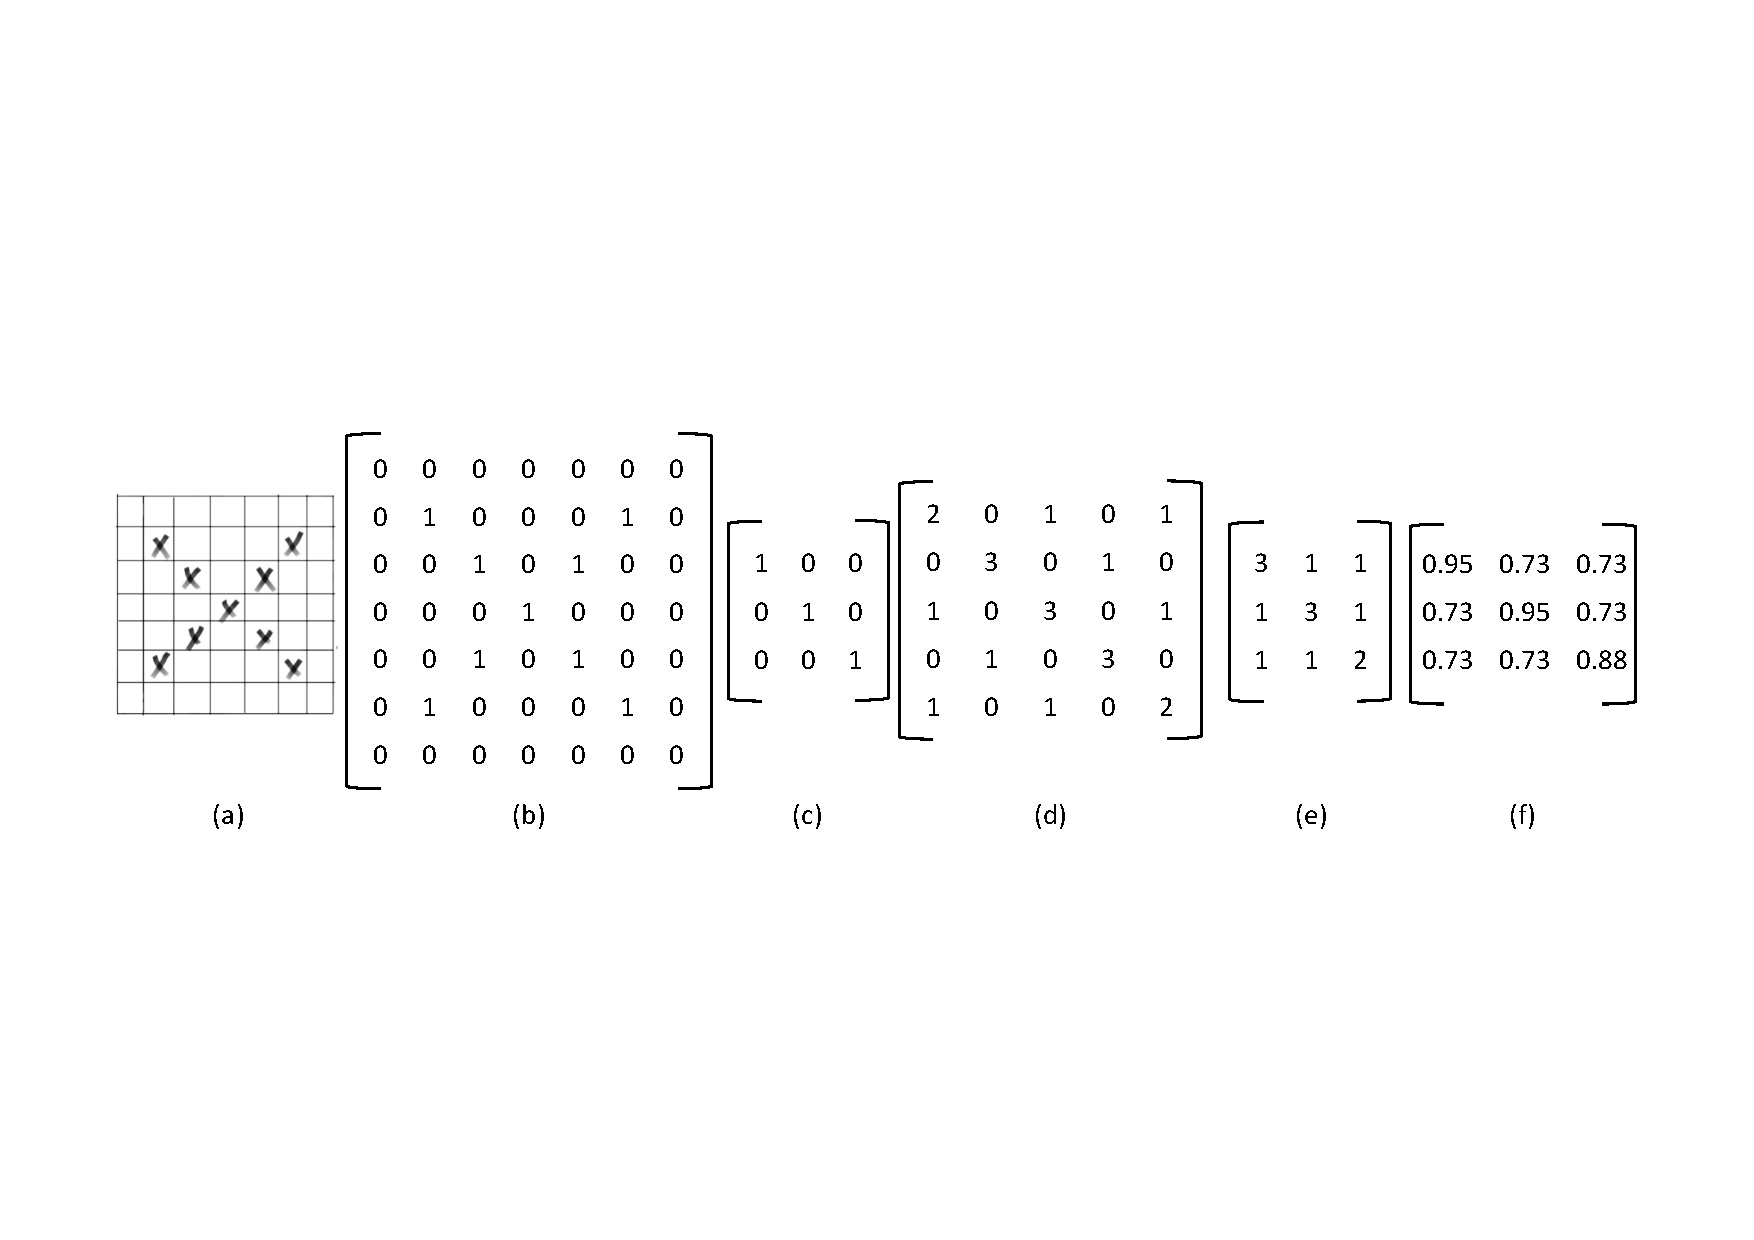
\includegraphics[width=7in]{img/X.pdf}
    \caption{From left to right: (a) Letter X in a 7x7 image; (b) Letter X in a 7x7 matrix; (c) A 3x3 convolution kernel; (d) A 5x5 feature map; (e) A 3x3 feature map after pooling; (f) A 3x3 feature map after activating with sigmoid function.}
    \label{X}
\end{figure*}




Neural networks originate from the human perception of the brain. In 1943, American neuroscientists McCulloch and Pitts proposed a theory that every neuron is a multiple-input single-output structure~\cite{mcculloch1943logical}. Furthermore, there are only two possibilities for this output signal: zero or one, which is very similar to a computer.

In image recognition, a 7x7 image, for example, has 49 elements or cells. If an `X' is written down in this grid, as shown in Figure~\ref{X}a, in the computer's view, it will be interpreted as a series of numbers (e.g. zeros and ones) as seen in Figure~\ref{X}b. If each cell is either black or white, for example, black can be assigned as one while white would be zero, resulting in a 7x7 matrix filled with zeros and ones. After feeding the algorithm as much data as available, it will be trained to find parameters to determine if the object is an `X' or not. For example, if it is a grey-scale picture, each number is not zero nor new, but instead a grey-scale value from 0 to 255. If it is a colour image, it will use the Red-Green-Blue (RGB) colours range. Essentially, no matter what the image is, the image can be interpreted as a combination number inside a matrix, this eventually working as the input of the neural network. The goal of training a neural network is to find the parameters that make the loss function - measures how far an estimated value is from its true value - smallest. However, the method described above is time-consuming and computationally expensive to train real-world images. Besides, the algorithm will be hard to recognise once the image is dilated, rotated or changed.


Based on the Neocognitron Model of Fukushima~\cite{fukushima1982neocognitron}, LeCun~\cite{lecun1995convolutional} invented a practical method for image recognition, called convolutional neural network. The role of convolution is to use a mathematical method to extract critical features from the image. The way to extract the features is to use a convolution kernel to do the convolution operation. The convolution kernel is a matrix, usually 3x3 or 5x5. For instance, if the convolution kernel is of the size 3x3, and the numbers in it are shown in Figure~\ref{X}c, then a convolution operation will be done with the 7x7 "X" matrix (Figure~\ref{X}b) and the kernel (Figure~\ref{X}c). The operation result of them is also known as a feature map (Figure~\ref{X}d)~\cite{bouvrie2006notes}.


The feature map reinforces the features of the convolution kernel, and this convolution kernel (the 3x3 convolution kernel in Figure~\ref{X}c) only has three oblique blocks of pixels being ones. So if the original 7x7 matrix (Figure~\ref{X}b) also has diagonal pixel blocks of ones, the number would be extensive when the convolution operation is done, which means the desired feature has been extracted. The smaller the value of the pixel block in the other positions of the feature map (Figure~\ref{X}d), the less it satisfies the feature. In general, different convolution kernels make it possible to get different feature maps.

The next step after convolution is pooling. The pooling method can reduce the feature map size and maintain similar features to the feature map before the pooling process. Figure~\ref{X}e shows the relatively small feature map after pooling the 5x5 matrix (Figure~\ref{X}d).


The step after pooling is activation. The activation function decides whether the neuron should be activated by computing the weighted sum and further adding the bias. The essence of the activation function is to introduce nonlinear factors to solve problems that a linear model cannot solve~\cite{lin2018research}. For example, after activating the sigmoid function, each element in the feature map would be between 0 to 1, as shown in Figure~\ref{X}f.

It is worth noting that the initial convolution kernel may be artificially set. Nevertheless, machine learning will go backwards to adjust and find the most suitable convolution kernel based on its data. Since an image generally has many features, there will be many corresponding convolution kernels. After many convolutions and poolings, features, including the diagonal lines of the image, the contours, and the colour features, can be found. This information is taken and fed into the fully connected network for training, and finally, it is possible to determine what this image is.


\subsection{Convolutional Neural Networks in Image Recognition}
\label{sec2.2}
The above literature review has demonstrated that past literature on shipping carbon inventories has not focused on small vessels. Thus the topic of activity-based emission inventories for this segment is an important gap in the literature. There is still considerable work to be done to understand how the small boat fleet operates, what fuels they are using, and the level of activity. However, with the development and maturation of a range of computer vision techniques such as convolutional neural networks (CNNs), it may be possible to accurately identify small vessels from open satellite imagery and support understanding of this ship segment. 

One of computer vision's most fundamental and challenging problems is target detection. The main goal of target detection is to determine the location of an object in an image based on a large number of predefined classes. Deep learning techniques, which have emerged in recent years, are a powerful method for learning features directly from data and have led to significant breakthroughs in the field of target detection. Furthermore, with the rise of self-driving cars and face detection, the need for fast and accurate object detection is growing.

In 2012, AlexNet, a deep convolutional neural network (DCNN) proposed by Krizhevsky et al.~\cite{krizhevsky2012imagenet}, achieved record accuracy in image classification at the ImageNet Large-Scale Visual Recognition Challenge (ILSRVC), making convolutional neural networks the dominant paradigm for image recognition. Then, Girshick et al.~\cite{girshick2014rich} introduce Region-Based Convolutional Neural Networks (R-CNN), the first convolutional neural network (CNN)-based object detection method. The R-CNN algorithm represents a two-step approach, where a region proposal is generated firstly, and then a CNN is used for recognition and classification. Compared to the traditional sliding convolutional window to determine the possible regions of objects, R-CNN uses selective search to pre-extract some candidate regions that are more likely to object to avoid computationally costly classification and object search, which makes it faster and significantly less computationally expensive~\cite{ uijlings2013selective, girshick2014rich}. Overall, the R-CNN approach is divided into four steps:

\begin{itemize}
    \item Generate candidate regions.
    \item Extract features using CNN on the candidate regions.
    \item Feed the extracted features into a Support Vector Machine (SVM) classifier.
    \item Correct the object positions by using a regressor.
\end{itemize}

However, R-CNN also has drawbacks: the selective search method is slow in generating positive and negative sample candidate regions for the training network, which affects the overall speed of the algorithm; R-CNN needs to perform feature extraction once for each generated candidate region separately; there are a large number of repeated operations which limits the algorithm performance ~\cite{huang2017speed}.

Since its inception, R-CNN has undergone several developments and iterations: Fast R-CNN, Faster R-CNN and Mask R-CNN~\cite{girshick2015fast, ren2015faster, he2017mask}. The improvement of Fast R-CNN is the design of a pooling layer structure for Region of Interest (ROI). The pooling stage effectively solves the R-CNN operation that crops and scales image regions to the same size, speeding up the algorithm. Faster R-CNN replaces the selective search method with Region Proposal Network (RPN) ~\cite{ren2015faster}. The selection and judgment of candidate frames are handed over to the RPN for processing, and the candidate regions are subjected to multi-task loss-based classification and localization processes. 

Several convolutional neural network-based object detection frameworks have recently emerged that can run faster, have a higher detection accuracy, produce cleaner results and are easier to develop. Compared to the Faster RCNN model, the YOLO model can detect better smaller objects, i.e. traffic lights at a distance~\cite{Dwivedi2020YOLOv5}, which is important when detecting objects in satellite images. Also, the YOLO model has a faster end-to-end run-time and detection accuracy than the Faster RCNN~\cite{Dwivedi2020YOLOv5}. Mask R-CNN upgrades the ROI Pooling layer of the Fast R-CNN to an ROI align layer and adds a branching FCN layer, the mask layer, to the bounding box recognition for semantic mask recognition~\cite{he2017mask}. Thus, the Mask R-CNN is essentially an Instance Segmentation algorithm, compared to Semantic Segmentation\footnote{In computer vision, image segmentation is the process of partitioning an image into multiple image segments, also known as image regions or image objects.}. Instance Segmentation is a more fine-grained segmentation of similar objects than Semantic Segmentation.

However, even traditional CNNs can be very useful for large-scale image recognition. For example, Simonyan and Zisserman~\cite{Simonyan2015VeryDC} researched the effect of convolutional network depth on its accuracy in large-scale image recognition settings. Their research found that even with small (3x3) convolution filters, significant accuracy is achieved by pushing the depth from 16 to 19 weight layers.

Finally, this study intends to develop the first stages of BoatNet. This image recognition model can detect small boats in any sea area, which in turn, and with further development, could significantly reduce the uncertainty in the estimation of the small boat fleet emission inventories in countries where the access to tracking infrastructure, costly satellite databases and labour-intensive methodologies are important barriers.



\section{ConvNet Configurations}
\label{chap:3}
\subsection{Target Areas in the Gulf of California and Dataset Statistical Analysis}
\begin{figure}[t]
    \center
    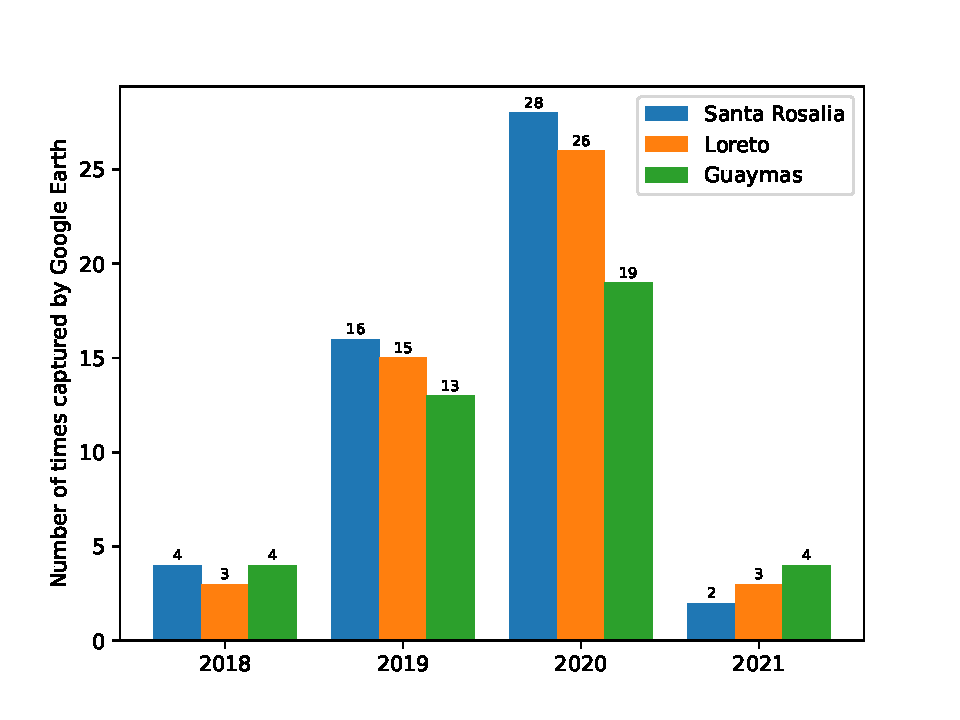
\includegraphics[width=\columnwidth]{img/NumberOfTimesCapturedByGEP.pdf}
    \caption{Number of times the three cities (Santa Rosalia, Loreto, Guaymas) captured by Google Earth Pro from 2018 to 2021.}
    \label{NumberOfTimesCapturedByGEP}
\end{figure}

The Gulf of California in Mexico was chosen as an area of study. Ideally, to analyze a sufficient amount of satellite image data, the ports of each of the major harbor cities in the Gulf of California would need to be included in the scope of our study. Thus, the first step in the work was to find out if there was enough satellite data for the area. In this study, we separate the Gulf of California into few parts on the Mexican state limits: (1) Baja California, (2) Sinaloa, (3) Sonora, (4) Baja California Sur. The satellite dataset used in this analysis includes 694 high-resolution images of ships around the world collected from Google Earth~\cite{lutherborrowship}. From the imagery dataset it was performed an statistical analysis on how many times, temporally speaking, the satellite database captured the region of interest. As a result of this analysis it was found out that:
\begin{itemize}
    \item most cities in the Gulf of California do not have enough satellite data in 2018 and in 2021 while many cities have relative rich satellite data between 2019 and 2020;
    \item there is a steady increase in the collection of satellite data in the Gulf of California from 2018 to 2020;
    \item the open-access and high-quality satellite data from Google Earth Pro is not immediately available for the public;
    \item differences in data accessibility are still evident among different cities. For example, it is accessible for some cities, like Guaymas in the state of Sonora, to have rich satellite images in 2019 and in 2020. However, some cities, such as La Ventana in the state of Baja California Sur, did not appear in Google Earth Pro in 2019 and 2020.
\end{itemize}

\begin{figure}[!t]
    \center
    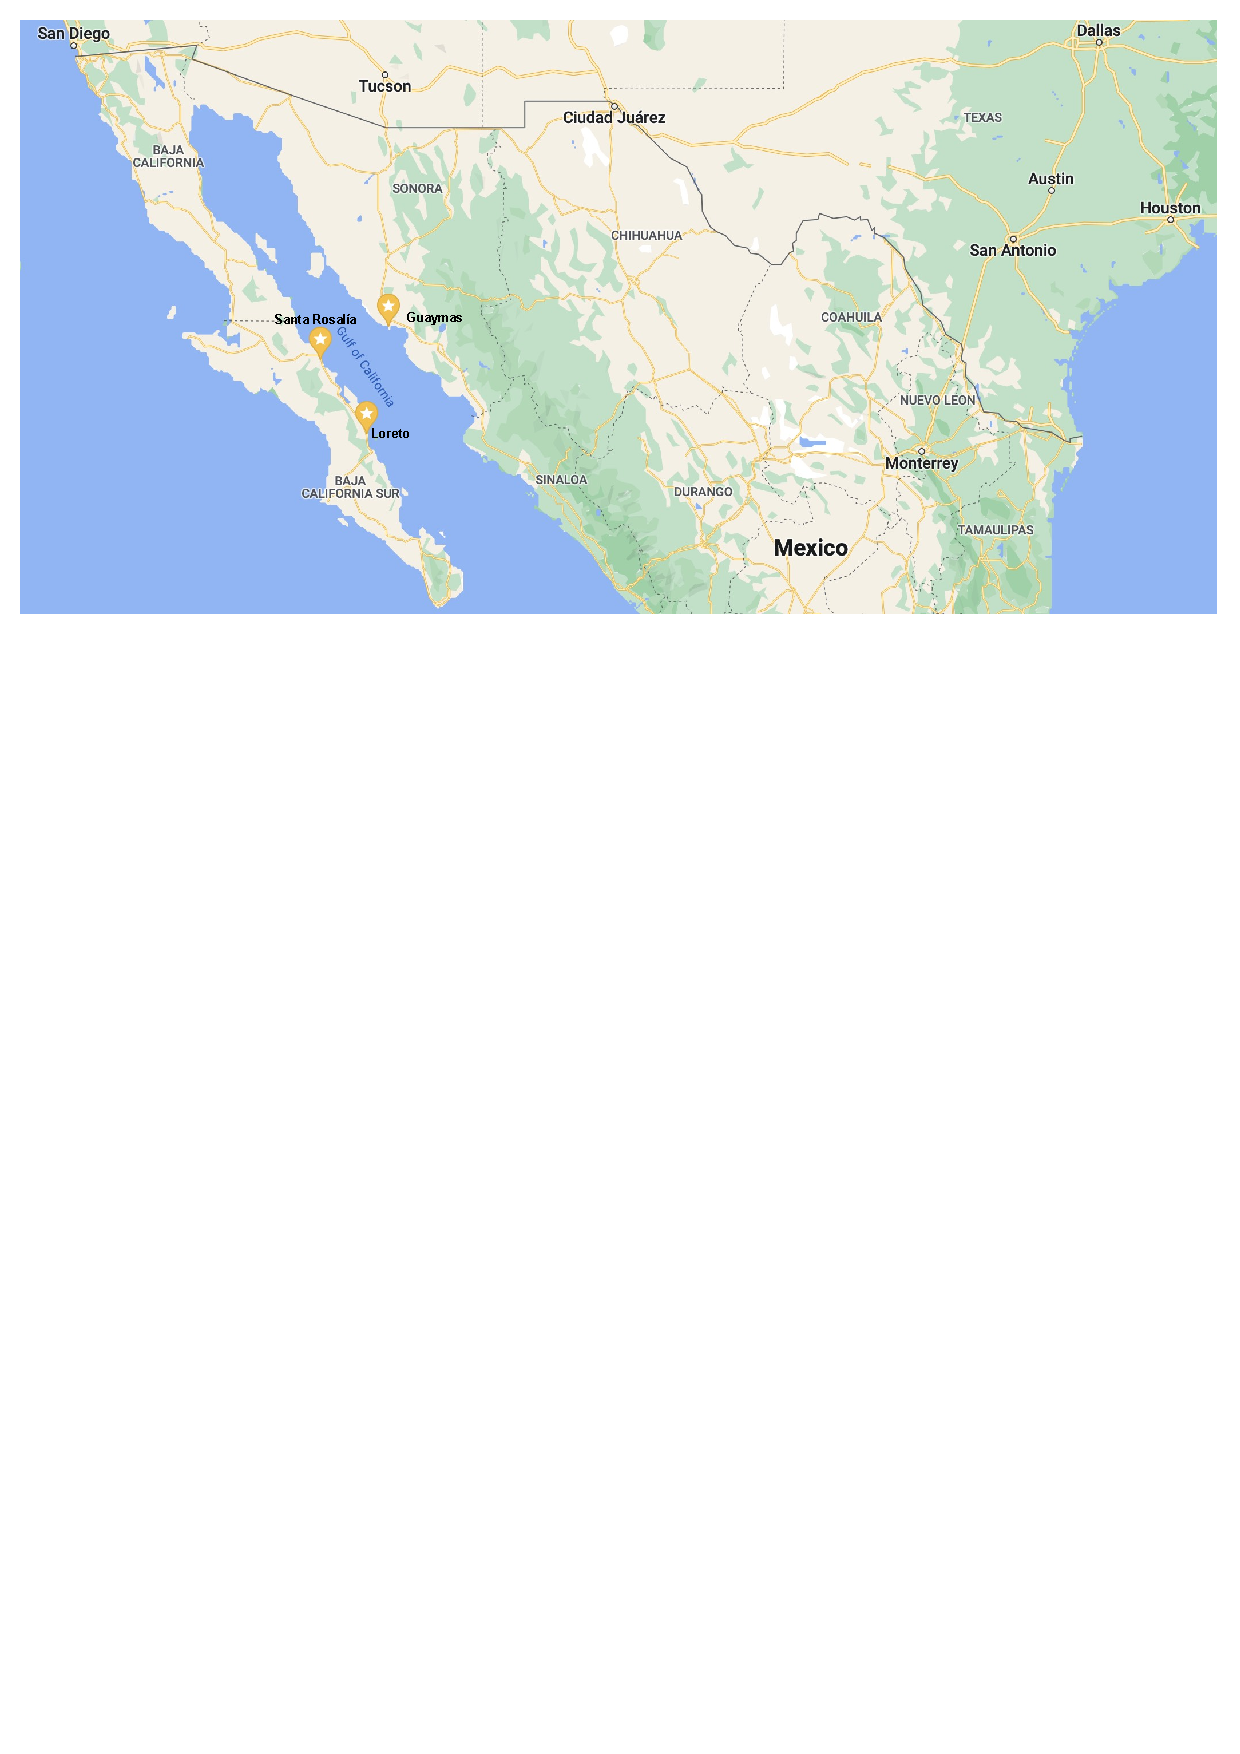
\includegraphics[width=\columnwidth]{img/locations_maps.pdf}
    \caption{The relative geographic locations of the three target cities - Santa Rosalia, Loreto, Guaymas - in Google Maps.}
    \label{locations_maps}
\end{figure}


For this reason, continuing with the previous strategy of analyzing the satellite data for each city in the Gulf of California would lead to a relatively large information bias and thus would not achieve an accurate result of the composition of the boats of the Gulf of California. Therefore, the following three cities with the richest data-accessibility in Google Earth Pro were chosen as the target areas for this study: Santa Rosalia, Loreto, Guaymas, of which the number of times captured by Google Earth Pro~\cite{lisle2006google} is shown in Figure~\ref{NumberOfTimesCapturedByGEP}. Relative geographic locations of the three target cities are shown in Figure~\ref{locations_maps}. The resulting database of the three Mexican coastal cities consisted of 583 images with timestamps between 2019 and 2020.


\subsection{Preprocessing}
Each satellite image was pre-labelled with a highly-precise label box manually~\cite{lutherborrowship}. The original dataset is contained images larger than 9 MB, which is an efficiency burden for the neural network training, especially when there are few objects to be detected. For this reason all the images were resized from 4800 pixels x 2908 pixels to 416 pixels x 416 pixels whose size is approximately 10 KB to 40 KB. 


\subsection{Single Object Detection Architecture}
\label{III-D-Detection-Architecture}

\begin{figure}[t]
    \center
    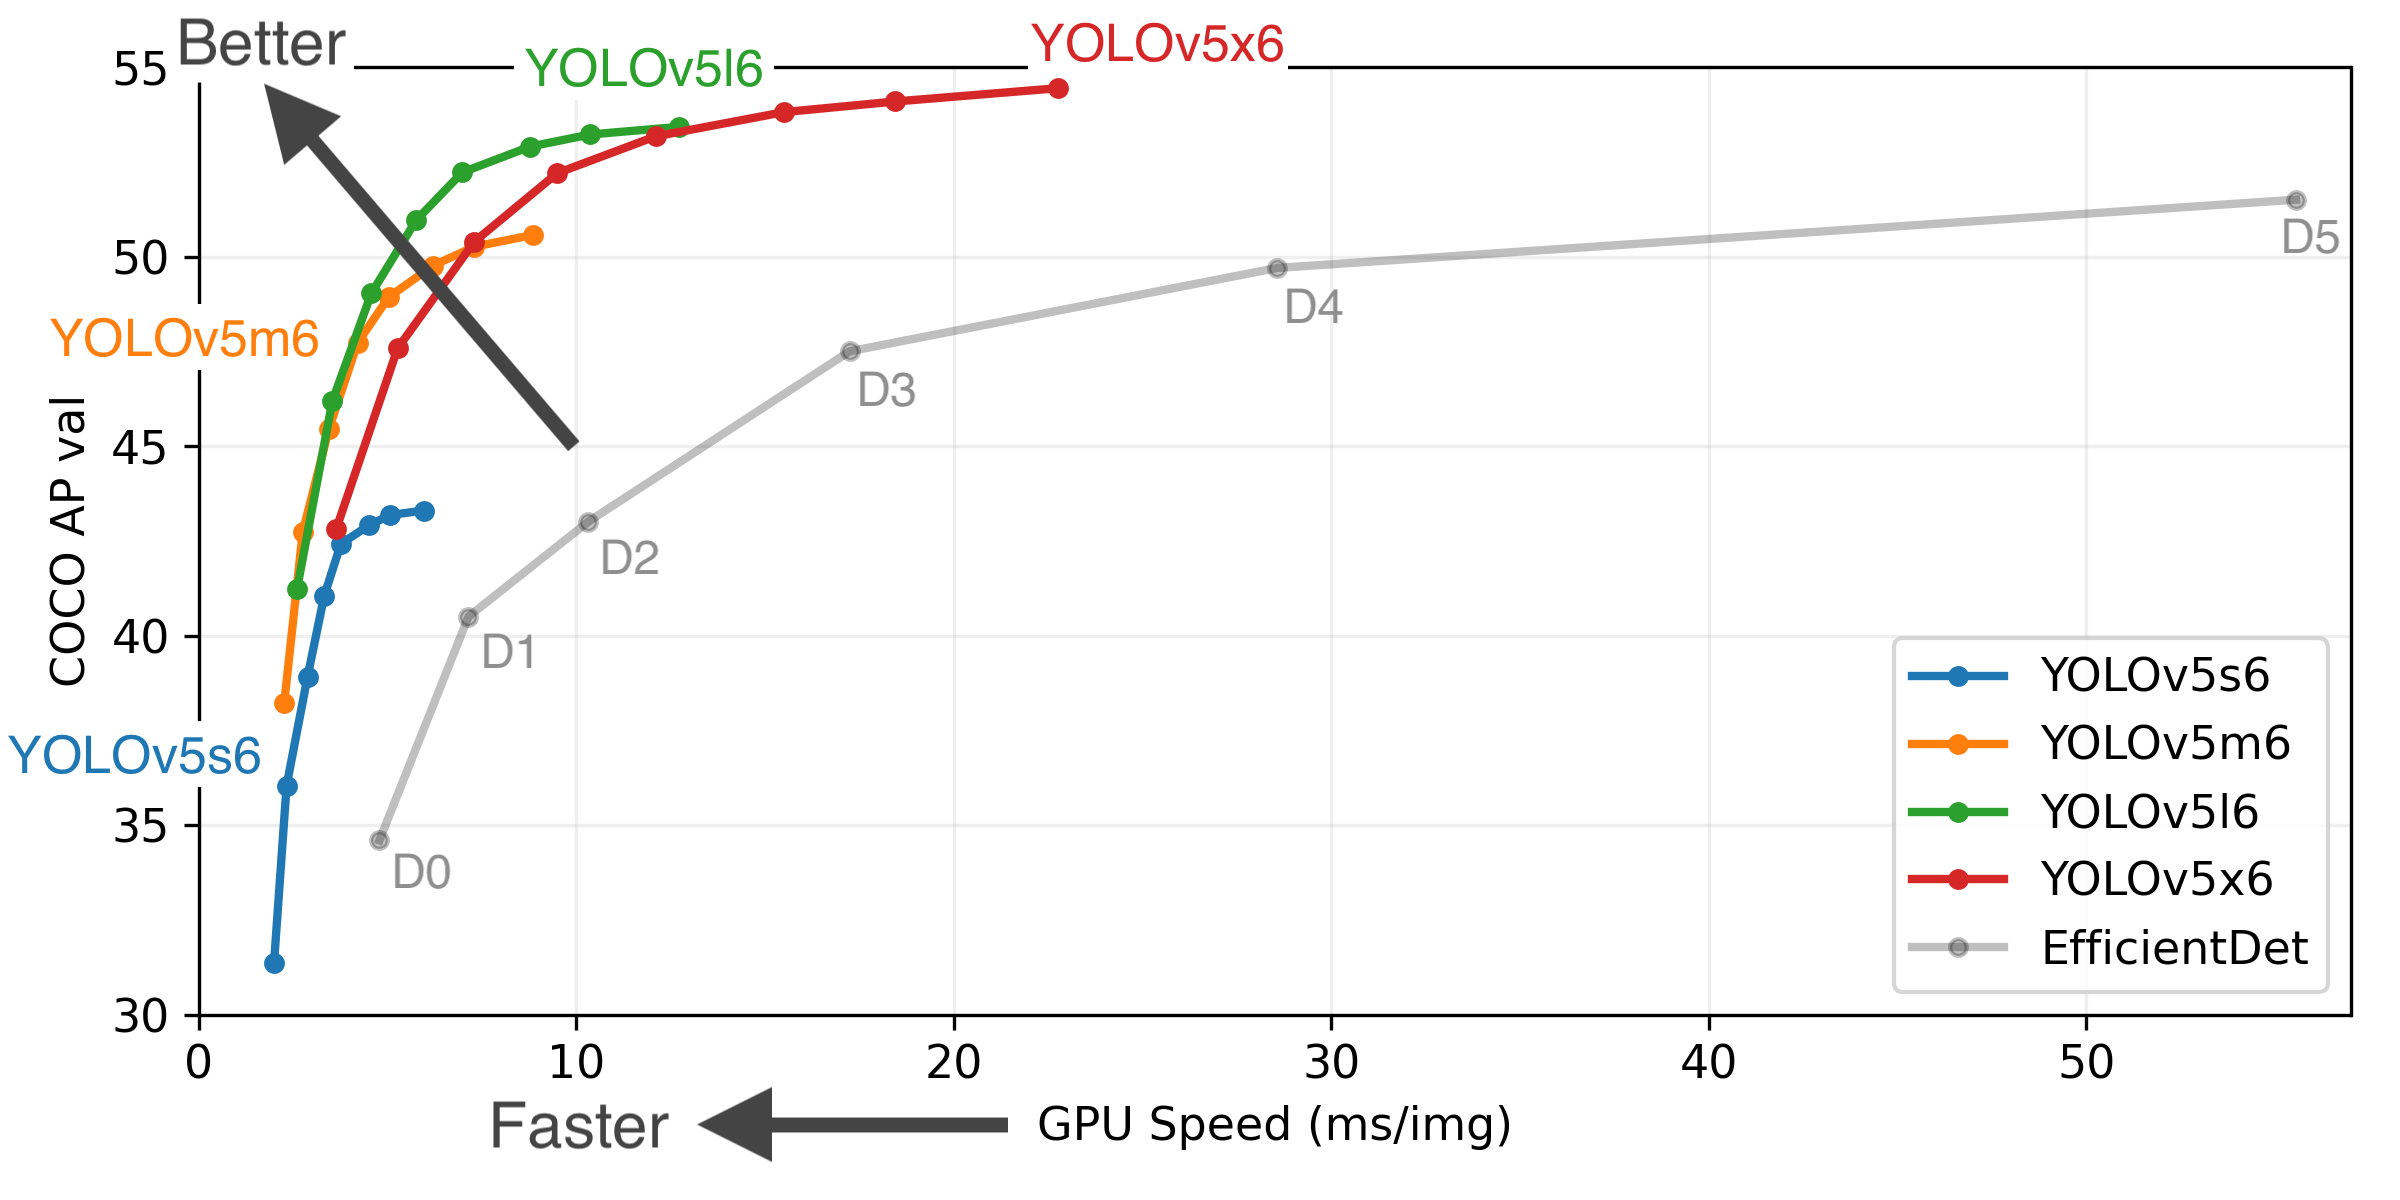
\includegraphics[width=\columnwidth]{img/YOLOv5_Performance.png}
    \caption{{Average Precision (AP) vs. GPU Speed in the 6th generation of YOLOv5 model under COCO data set~\cite{glenn_jocher_2020_4154370}.}}
    \label{fig:YOLOv5_Performance}
\end{figure}

\begin{figure*}[!t]
    \centering
    \includegraphics[width=7in]{img/model_architecture.pdf}
    \caption{\textbf{Model architecture.} Detection model architecture for obtaining a conclusion from an input satellite image of boats.  Images are preprocessed and passed through a CNN. The output of the model is a score, $y \in (0,1)$, representing the probability of being detected as a boat.}
    \label{model_architecture}
\end{figure*}


In Sec~\ref{sec2.2}, recent literature and development of Convolutional Neural Networks (CNNs), including the YOLO model, were discussed. YOLOv5 has four different categories of models, YOLOv5s, YOLOv5m, YOLOv5l, and YOLOv5x~\cite{glenn_jocher_2022_6222936}. They have 7.3 million, 21.4 million, 47.0 million and 87.7 million parameters, respectively. The performance charts can be seen as Figure~\ref{fig:YOLOv5_Performance} where the YOLOv5l model is able to achieve higher average precision with the same faster computing speed. Thus, in this study, the YOLOv5l model was chosen as the model for the training dataset. Figure~\ref{model_architecture} shows a schematic of the models being used for detecting boats, where satellite images in the Gulf of California are as the input of a pre-trained convolutional neural network (CNN). The detection accuracy was determined by computing the the mean probability score from the gulf's satellite images.

Satellite images often have noises, such as shadows cast by water on the sea surface due to sunlight or clouds in the atmosphere. These noises can make the training data inaccurate and often cause problems for the correctness of the model. He et al.~\cite{He2009SingleIH} proposed a simple but effective image prior-dark channel before removing haze from a single input image. The dark channel prior can be used as a statistics of outdoor haze-free images. Based on critical observation, most local patches in outdoor haze-free images contain some pixels whose intensity is very low in at least one color channel. Using this prior-dark channel before the haze imaging model, the thickness of the haze can be estimated, and a high-quality haze-free image can be recovered. Moreover, a high-quality depth map can also be obtained as a byproduct of haze removal.

Similar to the principle of using convolution kernels, specific image kernels can sharpen the image. While the sharpening kernel does not produce a higher resolution image, it emphasizes the differences in adjacent pixel values, making the image look more vivid. Overall, sharpening an image can significantly improve the recognition accuracy of an image with a 5x5 image kernel.

\subsection{Object Measurement and Classification}
Measuring the length of a ship is one of the most challenging topics in this study. As Google Earth Pro does not provide an application programming interface (API) for accurate scales, manually measuring the size of a particular scale became the core of measuring the size of a ship. In this work, all the captured satellite images were set with a fixed eye altitude. By measuring only one real length of the object through Google Earth measurement tool and knowing the pixel length of this object, the length of one pixel in the world of the fixed eye altitude can be calculated.

As the dataset for the training model was created with each edge tangent to the edge of the detected object, it can roughly treat the boat's length as the length of the diagonal of the detection box. Secondly, since the scale is central to the detection of the small boat fleet, the imagery scale should follow the following rules:
\begin{itemize}
    \item cannot be too large. The image needs to contain the full area where boats may be found.
    \item cannot be too small. If this is not follow it is highly probable that group of boats are detected as a single but larger boat.
    \item be sufficiently clear. This characteristic allows the algorithm to quantify the boat length and classified them accurately.
\end{itemize}


\begin{figure}[t]
    \centering
    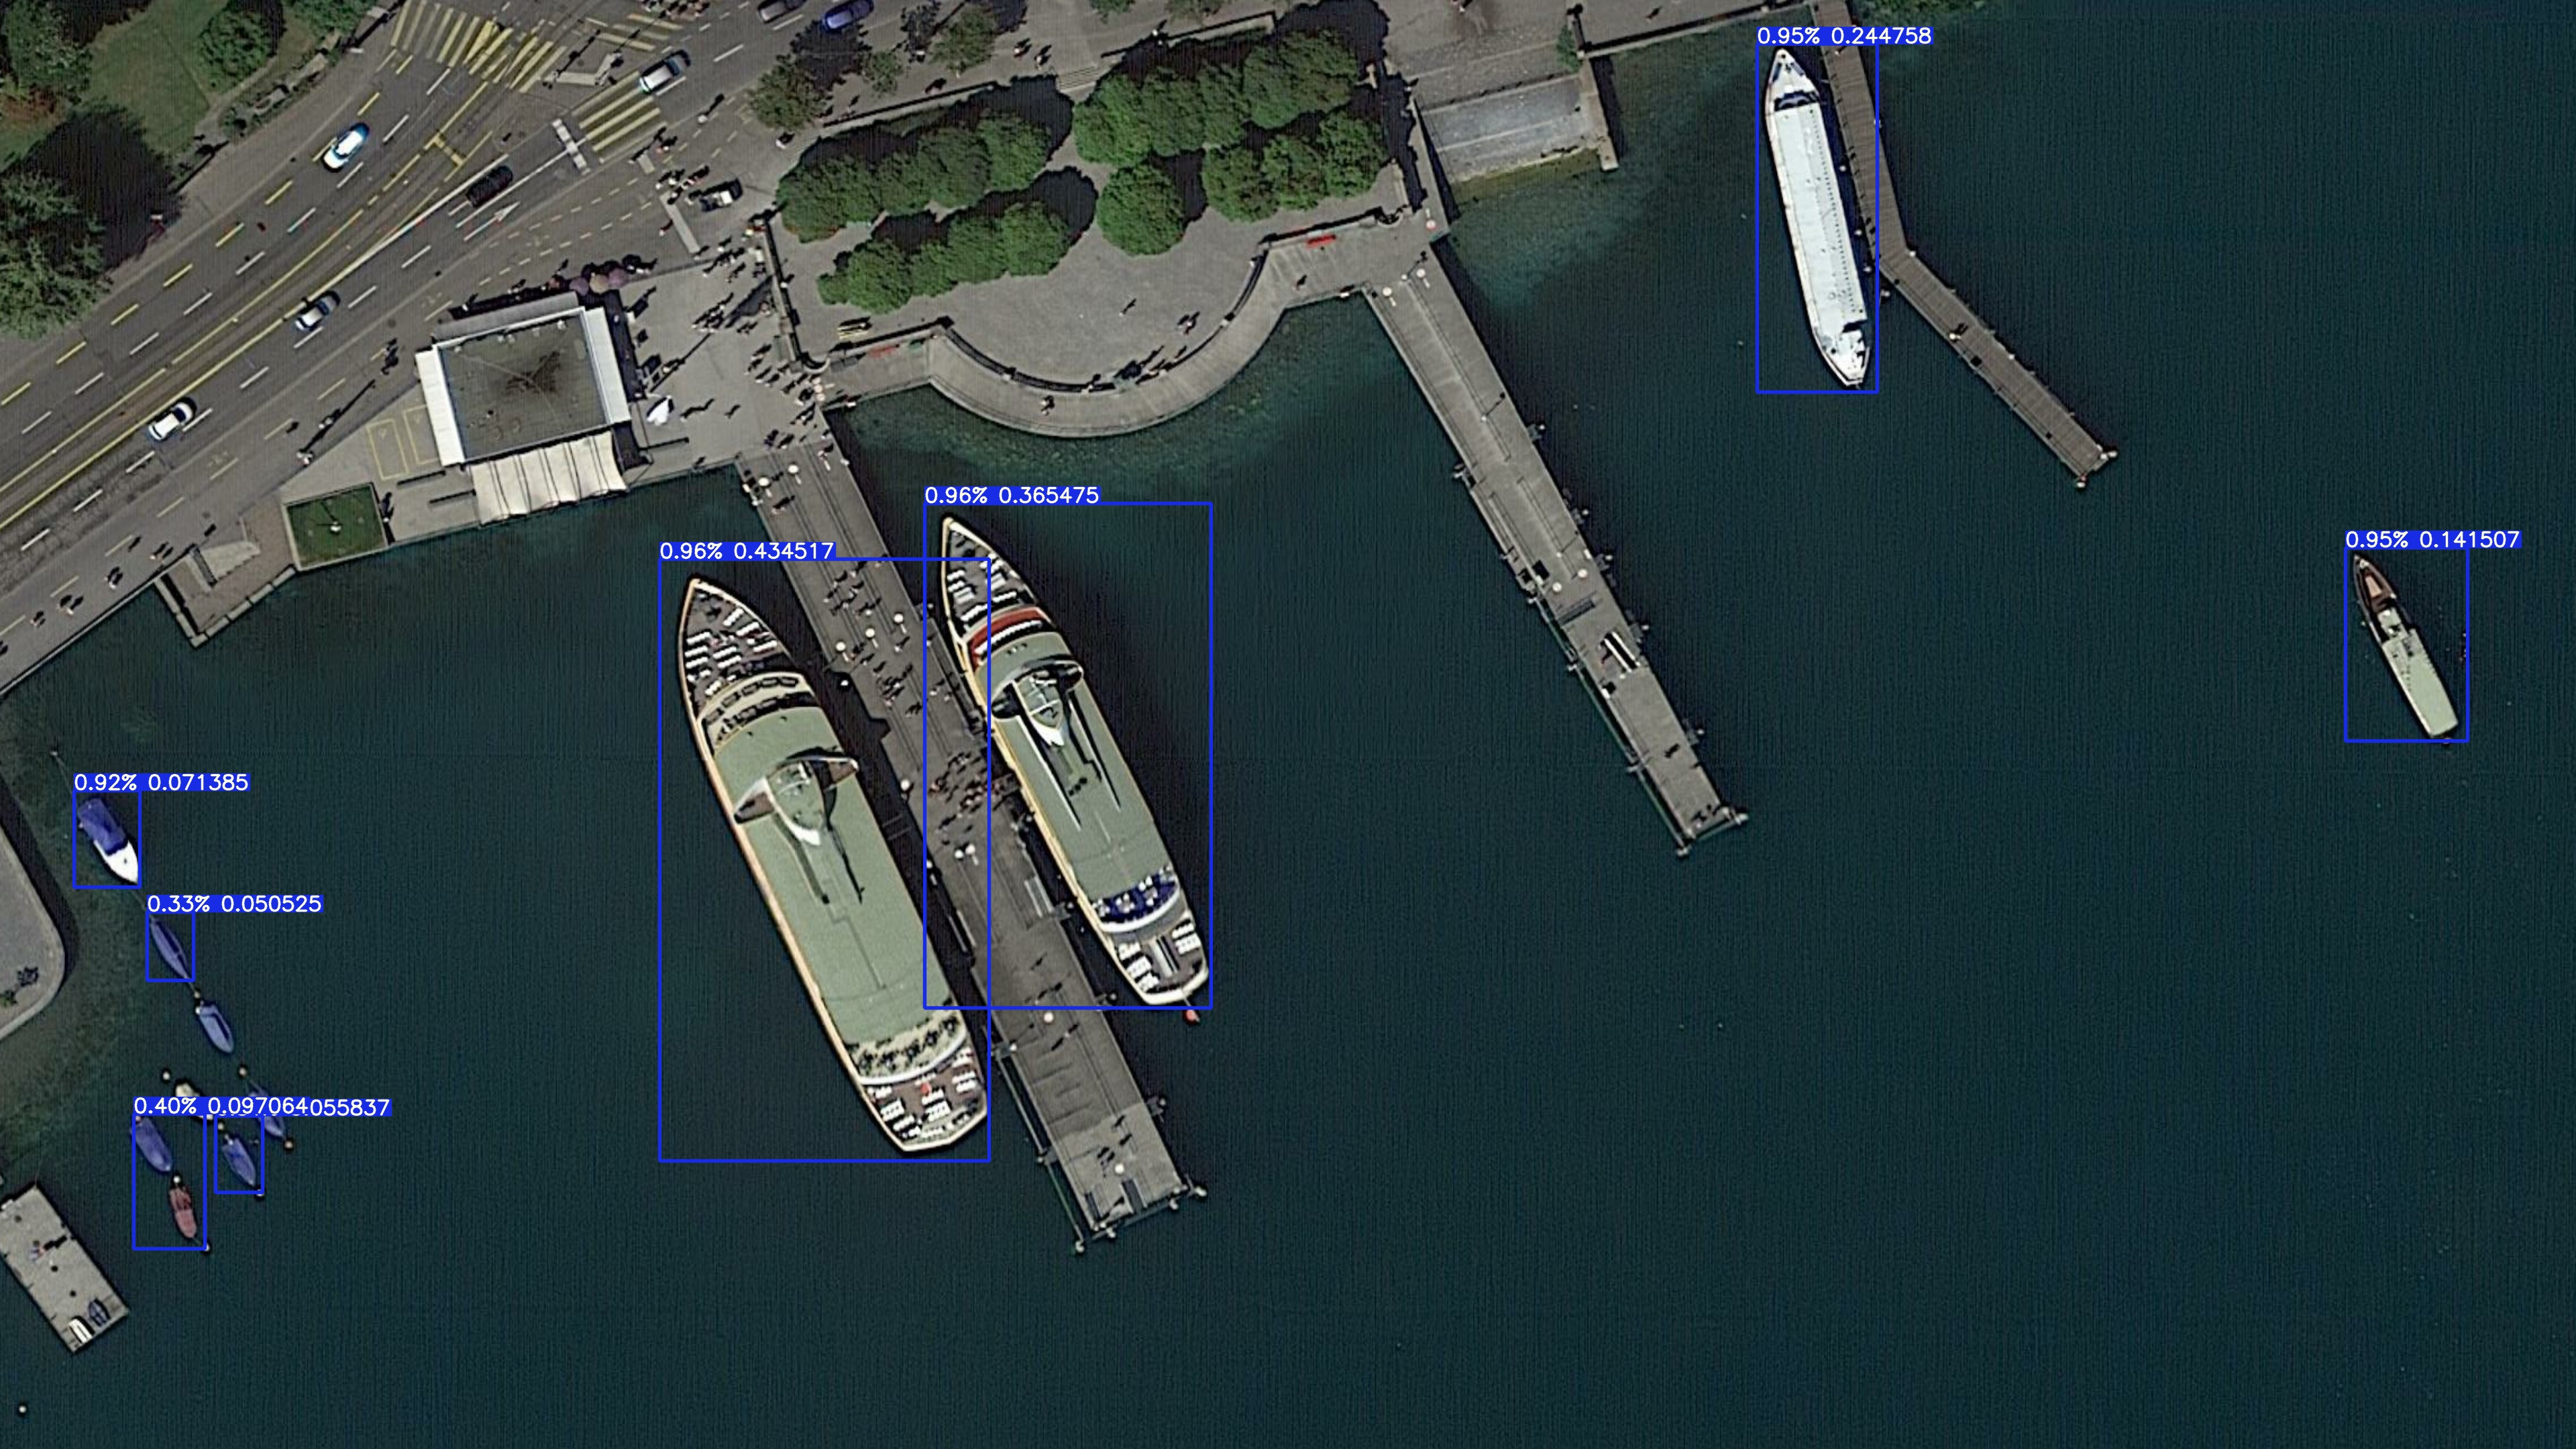
\includegraphics[width=\columnwidth]{img/zurich.jpeg}
    \caption{An image from Google Earth Pro for Zurich Lake on 16 Aug 2018 when eye alt is 200 meters.}
    \label{fig:zurich}
\end{figure}

Based on the above rules, the eye altitude was finally 200 meters. For this study it was used a satellite image of Zurich Lake, Switzerland, on 16th August 2018 as the standard image for defining the scale (Figure~\ref{fig:zurich}). Compared with other regions, the satellite image of Zurich Lake complies with the rules and it is a suitable candidate as the standard for measuring as a standard for measuring the length of small boats.

After measurement, the vessel in Figure~\ref{fig:zurich} had a YOLO length of 0.43 is 55.17 meters. Then, with an eye altitude of 200 meters, the ratio of the real length to the YOLO length is approximately 127. Finally, after several verifications, this ratio is within the margin of error and can be used as a scaling ratio. Moreover, having the same ratio and eye altitude is not enough. The resolution of each image needs to be the same so measurements are standardized. For this purpose, all datasets involved in the detection will maintain a resolution of 3840x2160 pixels which is the highest standard resolution in Google Earth.

In a certain sense, large vessels (e.g. cargo ships or warships) and small vessels (e.g. small boats for domestic use for recreation and fishing) are distinguished when creating the dataset for the area. However, due to the scaling, the eye altitude of the image is only 200 meters. Therefore, some large vessels, such as general cargo ships, do not even appear fully in an image, hence they are not considered in the statistical results of this work. On the other hand, some of the larger vessels, slightly shorter in length, are identified correctly by the algorithm and counted as part of the number of large vessels in the area. A Python script was then designed to count the number of small and large boats between regions.

After distinguishing between large and small boats, it is necessary to distinguish between small recreational boats for domestic use. For this work it was decided to start with two main categories, recreational boats and fishing boats without roof. To distinguish between them the model used the detected deck color of the the small boat. If the deck color was predominantly white then it was assigned as a recreational boat while any other mix of color will be assigned as a fishing both. It is recognized that this is a broad and simplistic classification method but it is an effective one to test the categorization power of the model. Each of the detected boats (i.e. the objects within the four coordinate anchor box) were analyzed whether the color was white or mainly white to then assign it to each category. As a final step the model performed the category counting for each image where a Python script was designed to count the small white boats.




\section{Results}
\label{chap:4}
\subsection{Train Custom Data: Weights, Biases Logging, Local Logging}

\begin{figure}[t]
    \centerline{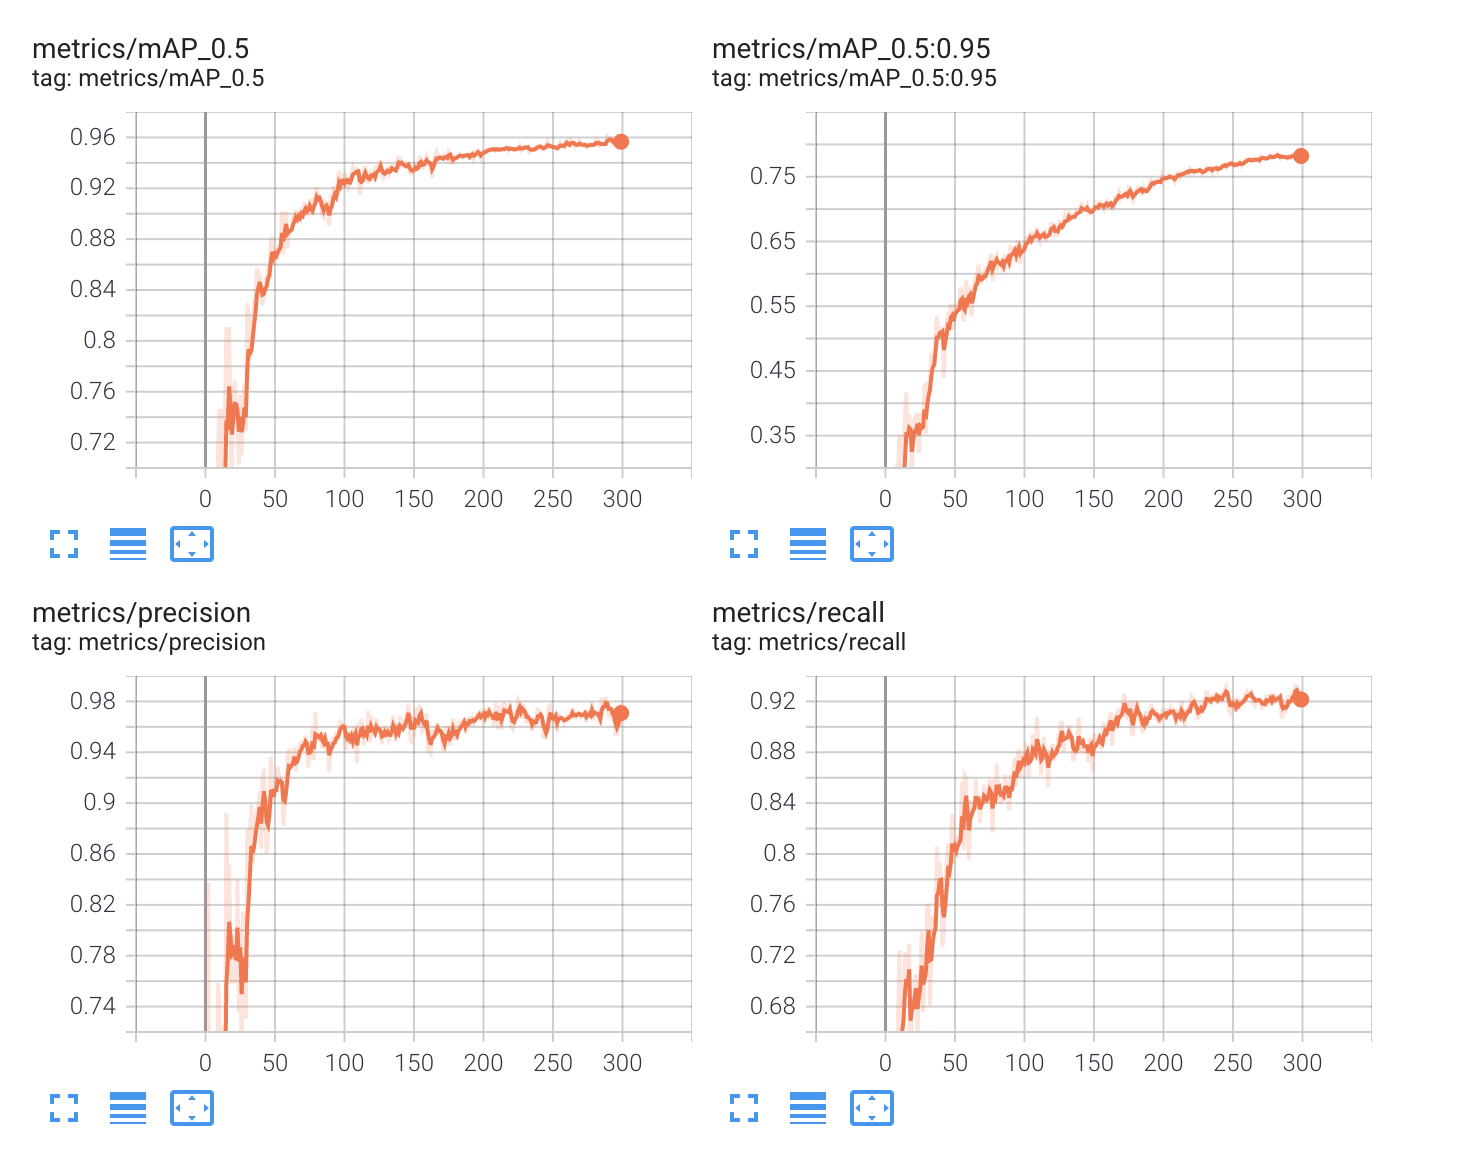
\includegraphics[width=\columnwidth]{img/colab_metrics.png}}
    \caption{Average model precision when IOU is larger than 0.5; Average model precision when IOU is between 0.5 and 0.95; The model precision; The model recall rate.}
    \label{fig:colab_metrics}
\end{figure}

\begin{figure}[t]
    \centerline{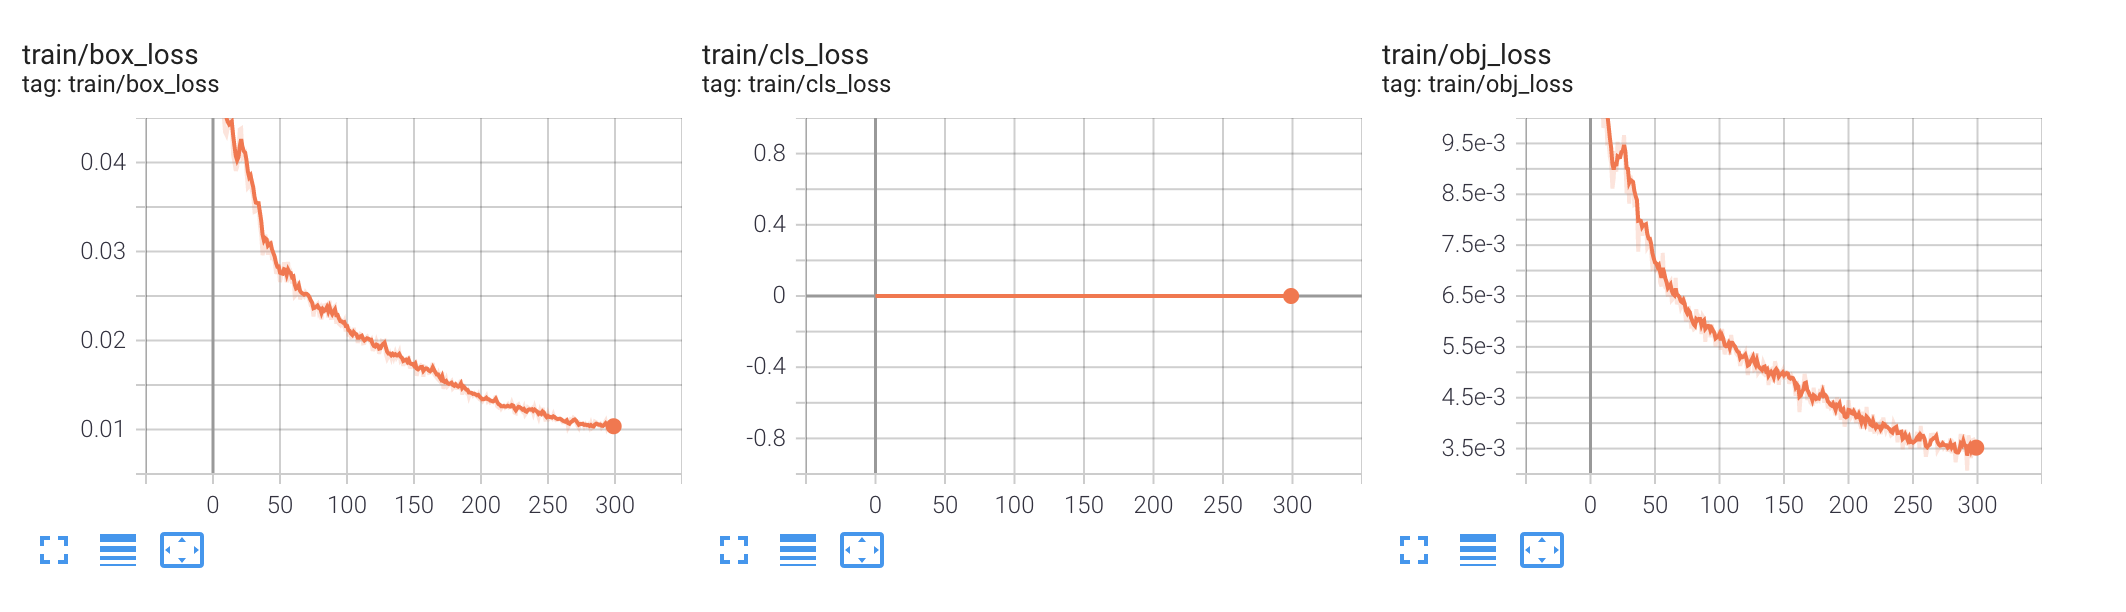
\includegraphics[width=\columnwidth]{img/colab_train.png}}
    \caption{The box loss rate of the model; The class loss rate of the model; The object loss rate of the model.}
    \label{fig:colab_train}
\end{figure}

\begin{figure}[t]
    \centerline{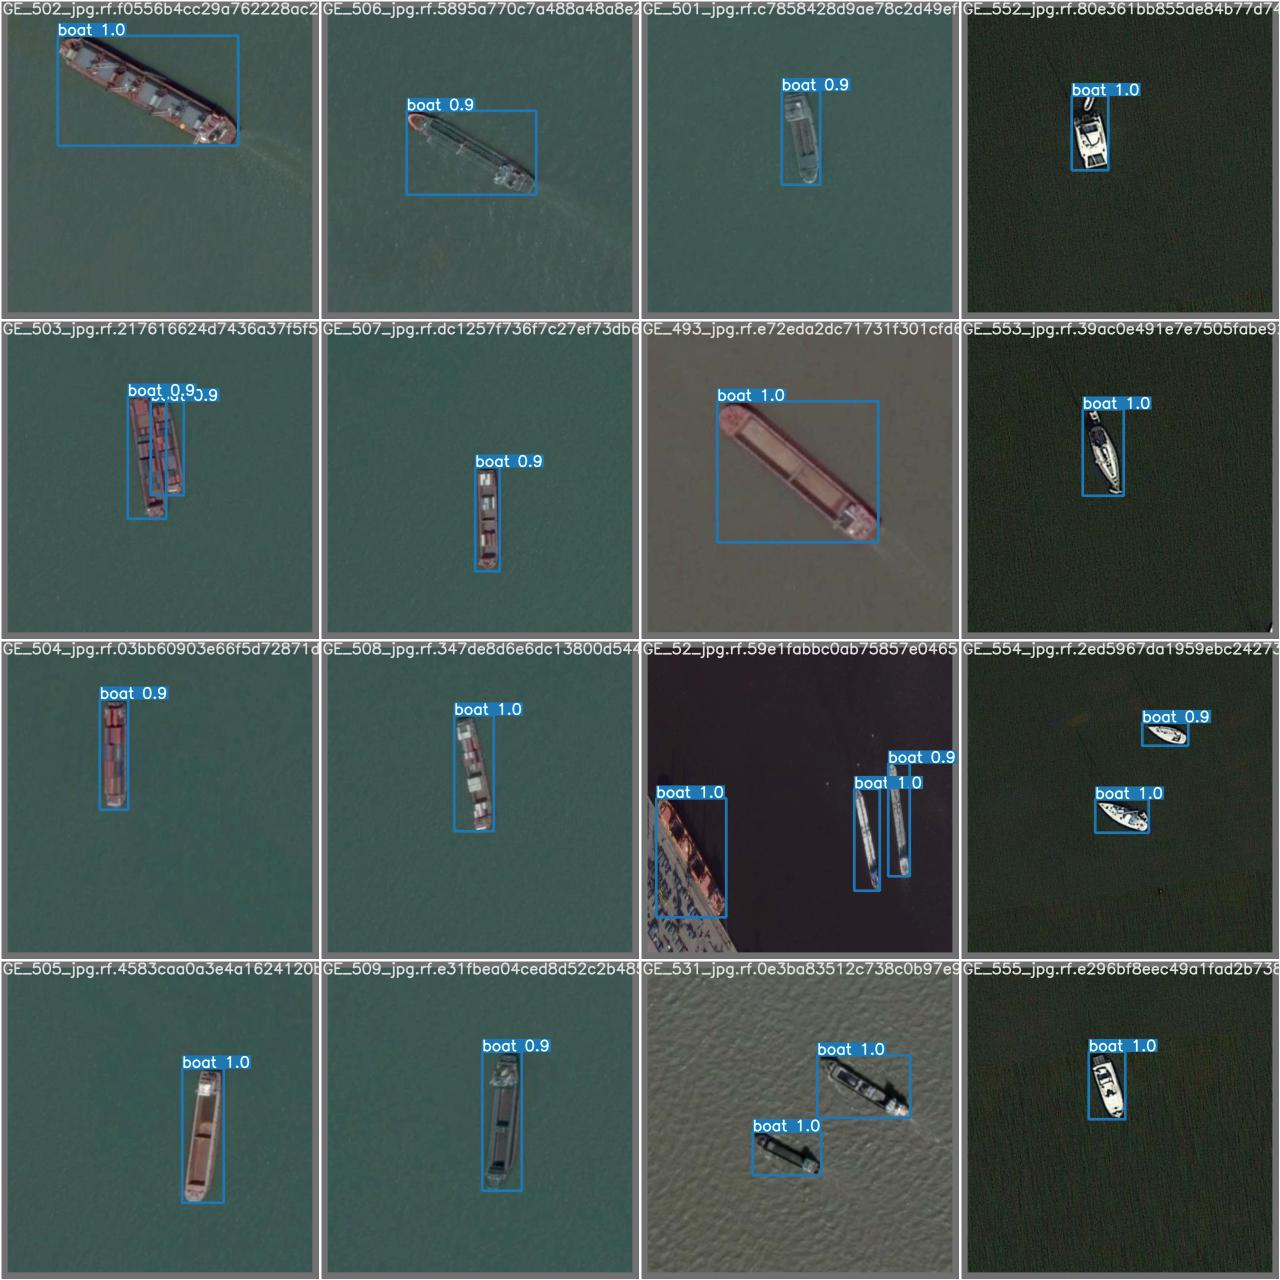
\includegraphics[width=\columnwidth]{img/test_batch1_pred.jpeg}}
    \caption{Test result of a trained model for detecting ships.}
    \label{fig:test_batch1_pred}
\end{figure}

As shown in Figure~\ref{fig:colab_metrics}, the average accuracy of the model, precision, and recall of the model all show a significant increase with the number of model training when the Intersection Over Union (IOU)\footnote{IOU is an evaluation metric used to measure the accuracy of an object detector on a particular dataset.} is between 50\% and 95\%. In particular, the precision of the model can eventually reach a level close to 96\%. However, this does not necessarily mean that the model will also fit satellite imagery of the Gulf of California. First, such high accuracy results only tell us that the model can achieve a relatively high recognition accuracy, which gradually increases and reaches 96\% after 300 training repetitions. If the algorithm needs to be trained for this area, then consideration must be given to purposefully selecting many small boats in or near the area as a data source for training the model. 

To train models faster, we reduced the images' resolution by about 70, which leaves images of 416 pixels x 416 pixels. Otherwise, the training could take half a month if the used images had a resolution of 4800 pixels x 2908 pixels.

Similarly, as shown in Figure~\ref{fig:colab_train}, the loss rate of the box can eventually reach 1\% as the number of training sessions increases. Since this study has defined only one class of object (i.e. boat), the probability that the detection box does not detect that it is a boat at all is 1\%. Similarly, because there is only one class, the class loss rate is 0. Figure~\ref{fig:test_batch1_pred} shows the prediction results during the training of the model, and it can be seen that the model can detect the presence of vessels in 100\% of the tested ranges and give the corresponding range boxes. Most detected boats have a 90\% probability of being boats, an acceptable value for object detection. Since only one class was set, some were also considered a 100\% probability of being boats.

\subsection{Detection Results and Small Boat Composition}
Starting with the length measurement comparison of a detected small boat and a large ship by BoatNet against Google Earth Pro measuring tools, Figure~\ref{fig:length_test} shows that the small boat detected measured 6.98 meters using Google Earth Pro while BoatNet estimated 6.74 meters. The error between them is 3.4\%. Google Earth Pro measured the larger ship at 41.38 meters and BoatNet at 40.98 meters. The error between them is less than 1.0\%.

\begin{figure}[t]
    \center
    \includegraphics[width=\columnwidth]{img/length_test.png}
    \caption{Compare the length of boats using Google Earth ruler and computer vision algorithm. For example, it is the image from Google Earth Pro for Zurich Lake on 16th August 2018 when the eye alt is 200 meters.}
    \label{fig:length_test}
\end{figure}

As explained in Sec~\ref{III-D-Detection-Architecture}, it was unproductive for the model to select the entire region for the study due to the varying amount of publicly available regional images from Google Earth Pro over the past three years. Ultimately, the satellite images database was built of 690 images. However, as stated in Sec~\ref{III-D-Detection-Architecture}, some of the slightly earlier satellite images had inferior detail representation capabilities, which resulted in the model not being very good at accurately detecting the features of the target. To improve the model accuracy, an image enhancement process using a 5x5 sharpening kernel allowed for a higher recognition rate. However, the following situations still occur:

\begin{enumerate}
    \item Figure~\ref{fig:1_docked_together_Guaymas_202001_20}: When the detailed representation of the image is indigent, i.e., the images are blurred, and two or three small boats are moored together, the model is very likely to recognise the two or three boats as a whole. There are two reasons for this problem. First, the training data is primarily a 'fuzzy' data source. Thus, when two or three small boats moored together, the model cannot easily detect the features of each small boat individually. In contrast, it may seem more reasonable to the model that the two or three boats as a whole have the same features. The second reason is that most data sources are individual boats on the surface or boats docked close to each other. As the data sources do not fully consider the fuzzy nature of the detail needed to detect the object and the fact that they are too close together, the model naturally does not recognise such cases.

    
    \item Figure~\ref{fig:2_square_Guaymas_202001_01}: When a large cargo ship is moored, the ship appears as a 'rectangle' from the air, much like a long pier, and is sometimes undetectable because small vessels with a rectangular shape were not common at the time data feed was compiled. This also applies to uncommon vessels such as battleships. This could be corrected if the model considered larger ships, but this was outside the scope of this work.

    \item Figure~\ref{fig:3_beach_SantaRosalia_202104_02}: The recognition rate was also significantly lower when the boats sometimes lay on the beach rather than floating on the water. This is because most of the training data are based on images in the water rather than the boats on the beach.

\end{enumerate}

\begin{figure}[t]
    \centering
    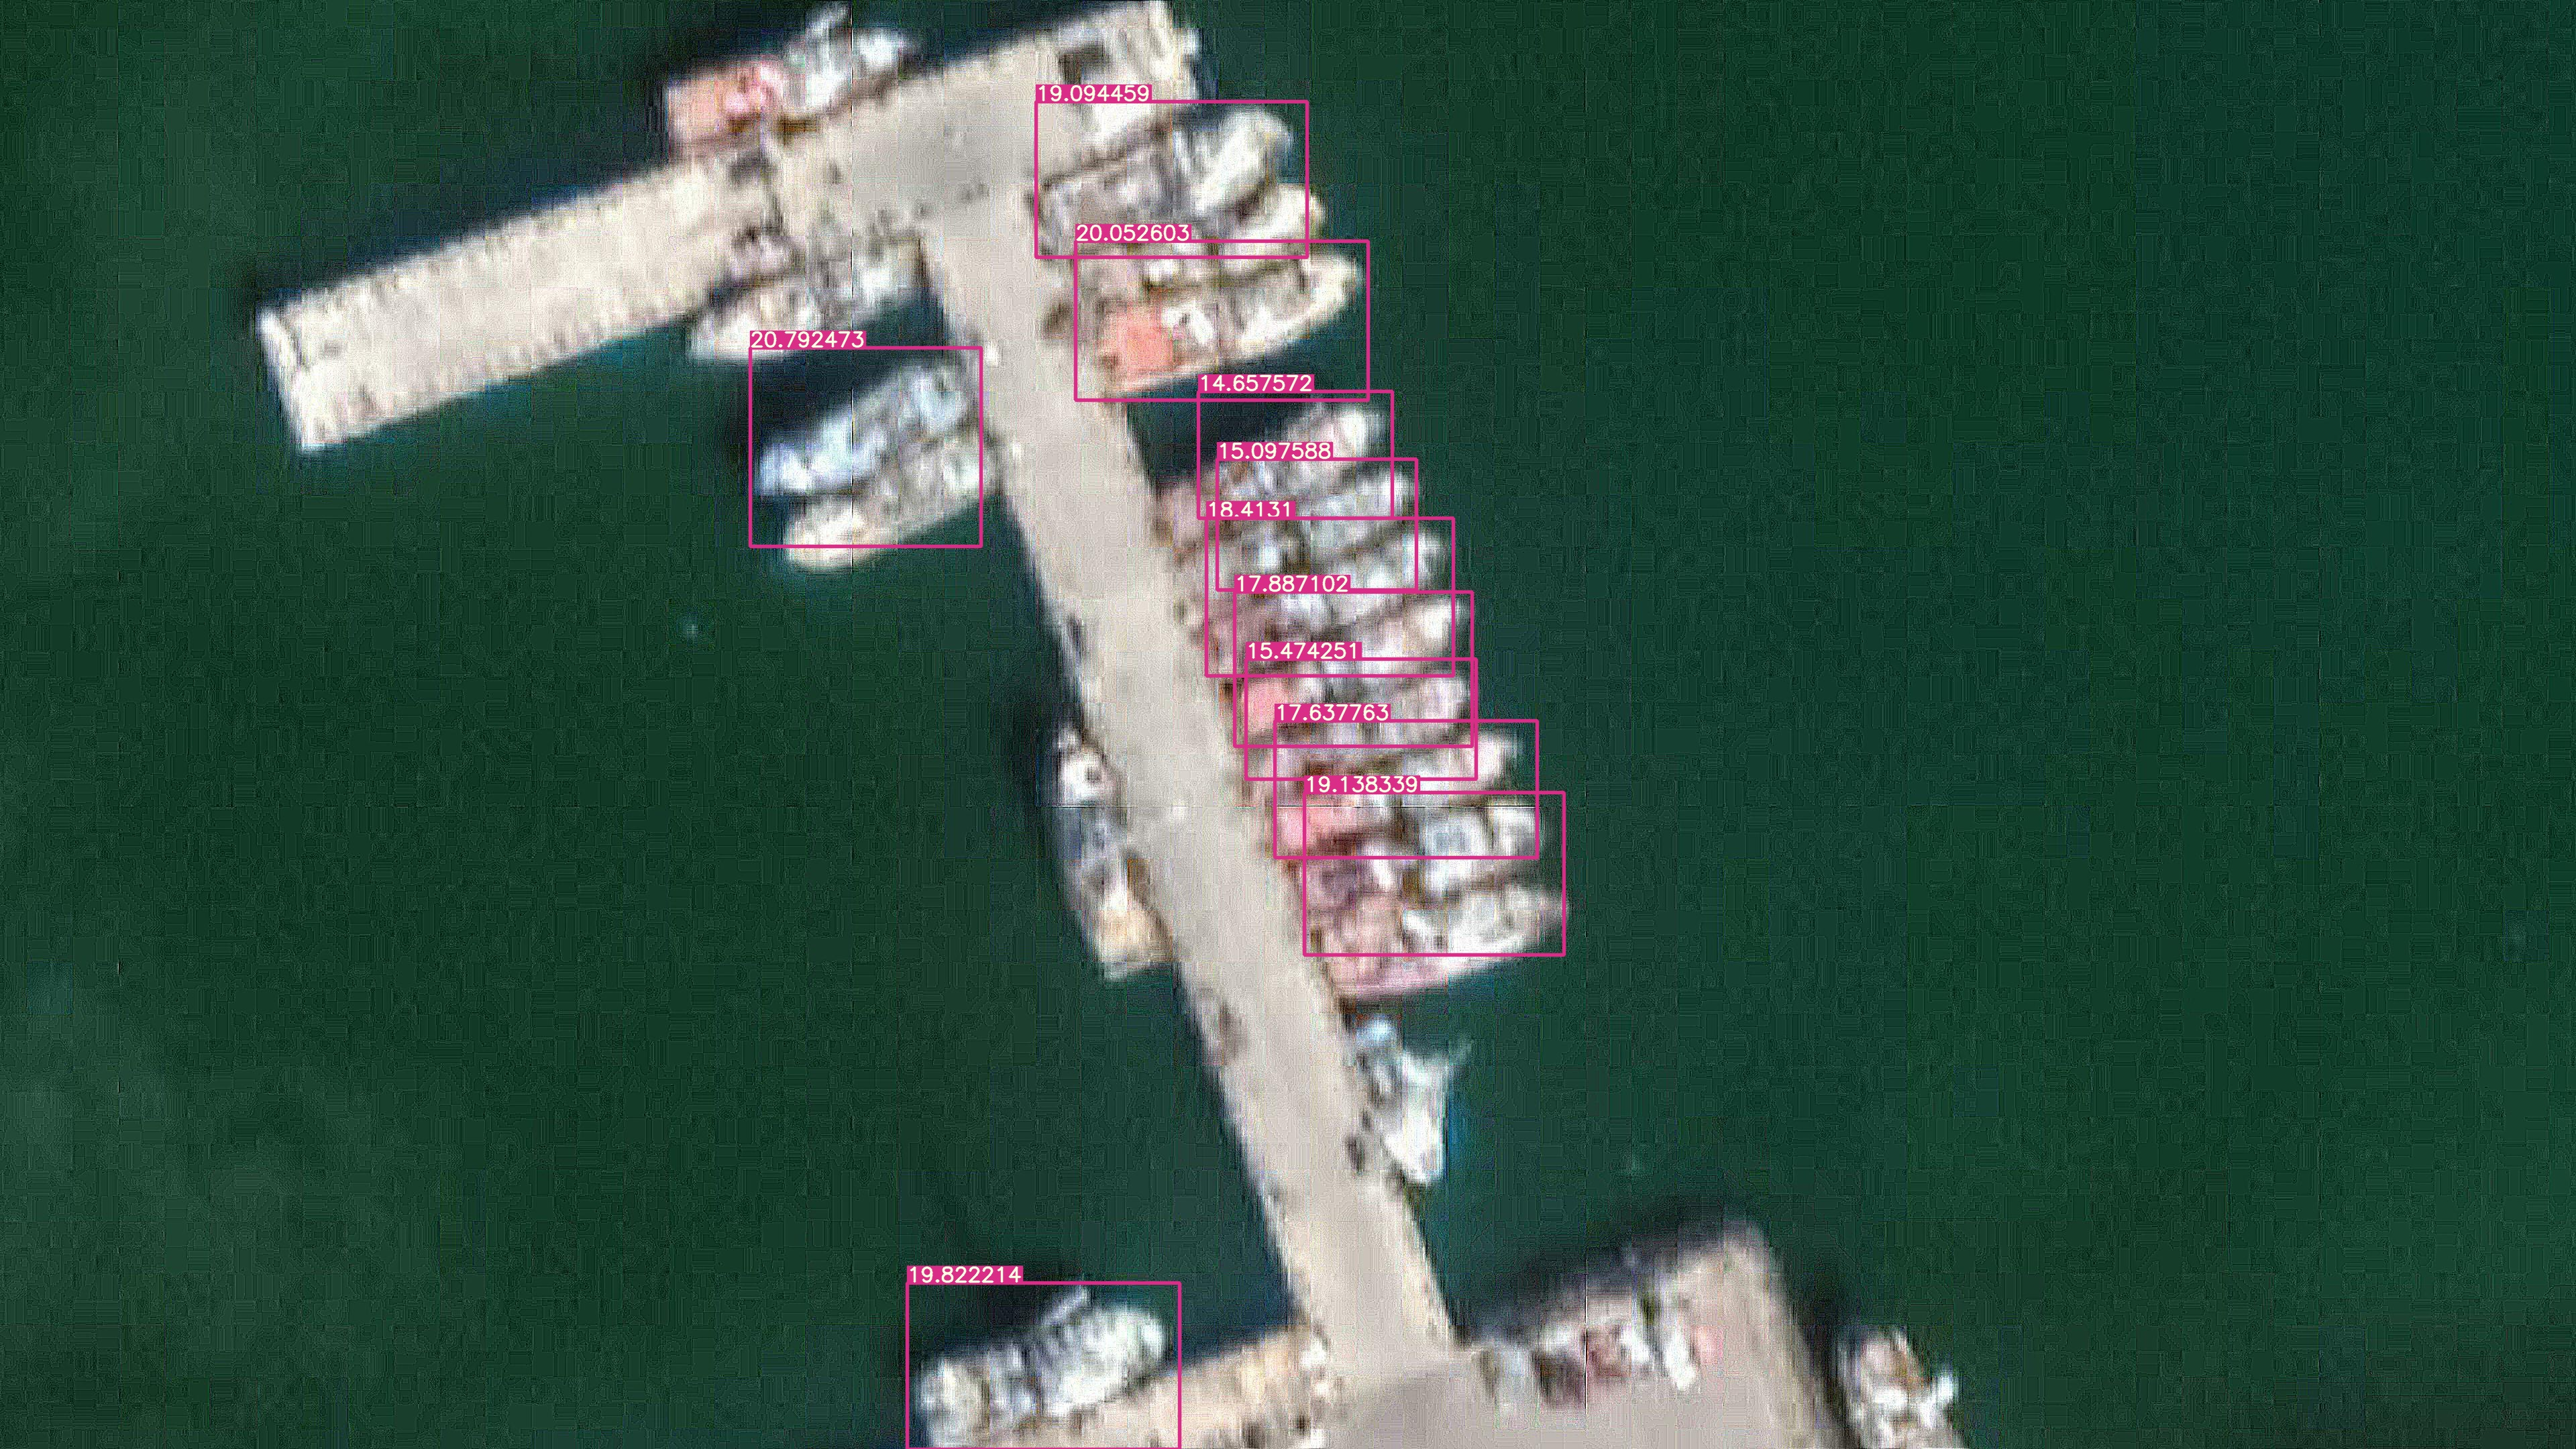
\includegraphics[width=\columnwidth]{img/1_docked_together_Guaymas_202001_20.jpeg}
    \caption{When small boats are moored closely together in the harbour, the model may recognise two small boats as one. The image is from Guaymas, January 2020.}
    \label{fig:1_docked_together_Guaymas_202001_20}
\end{figure}

\begin{figure}[t]
    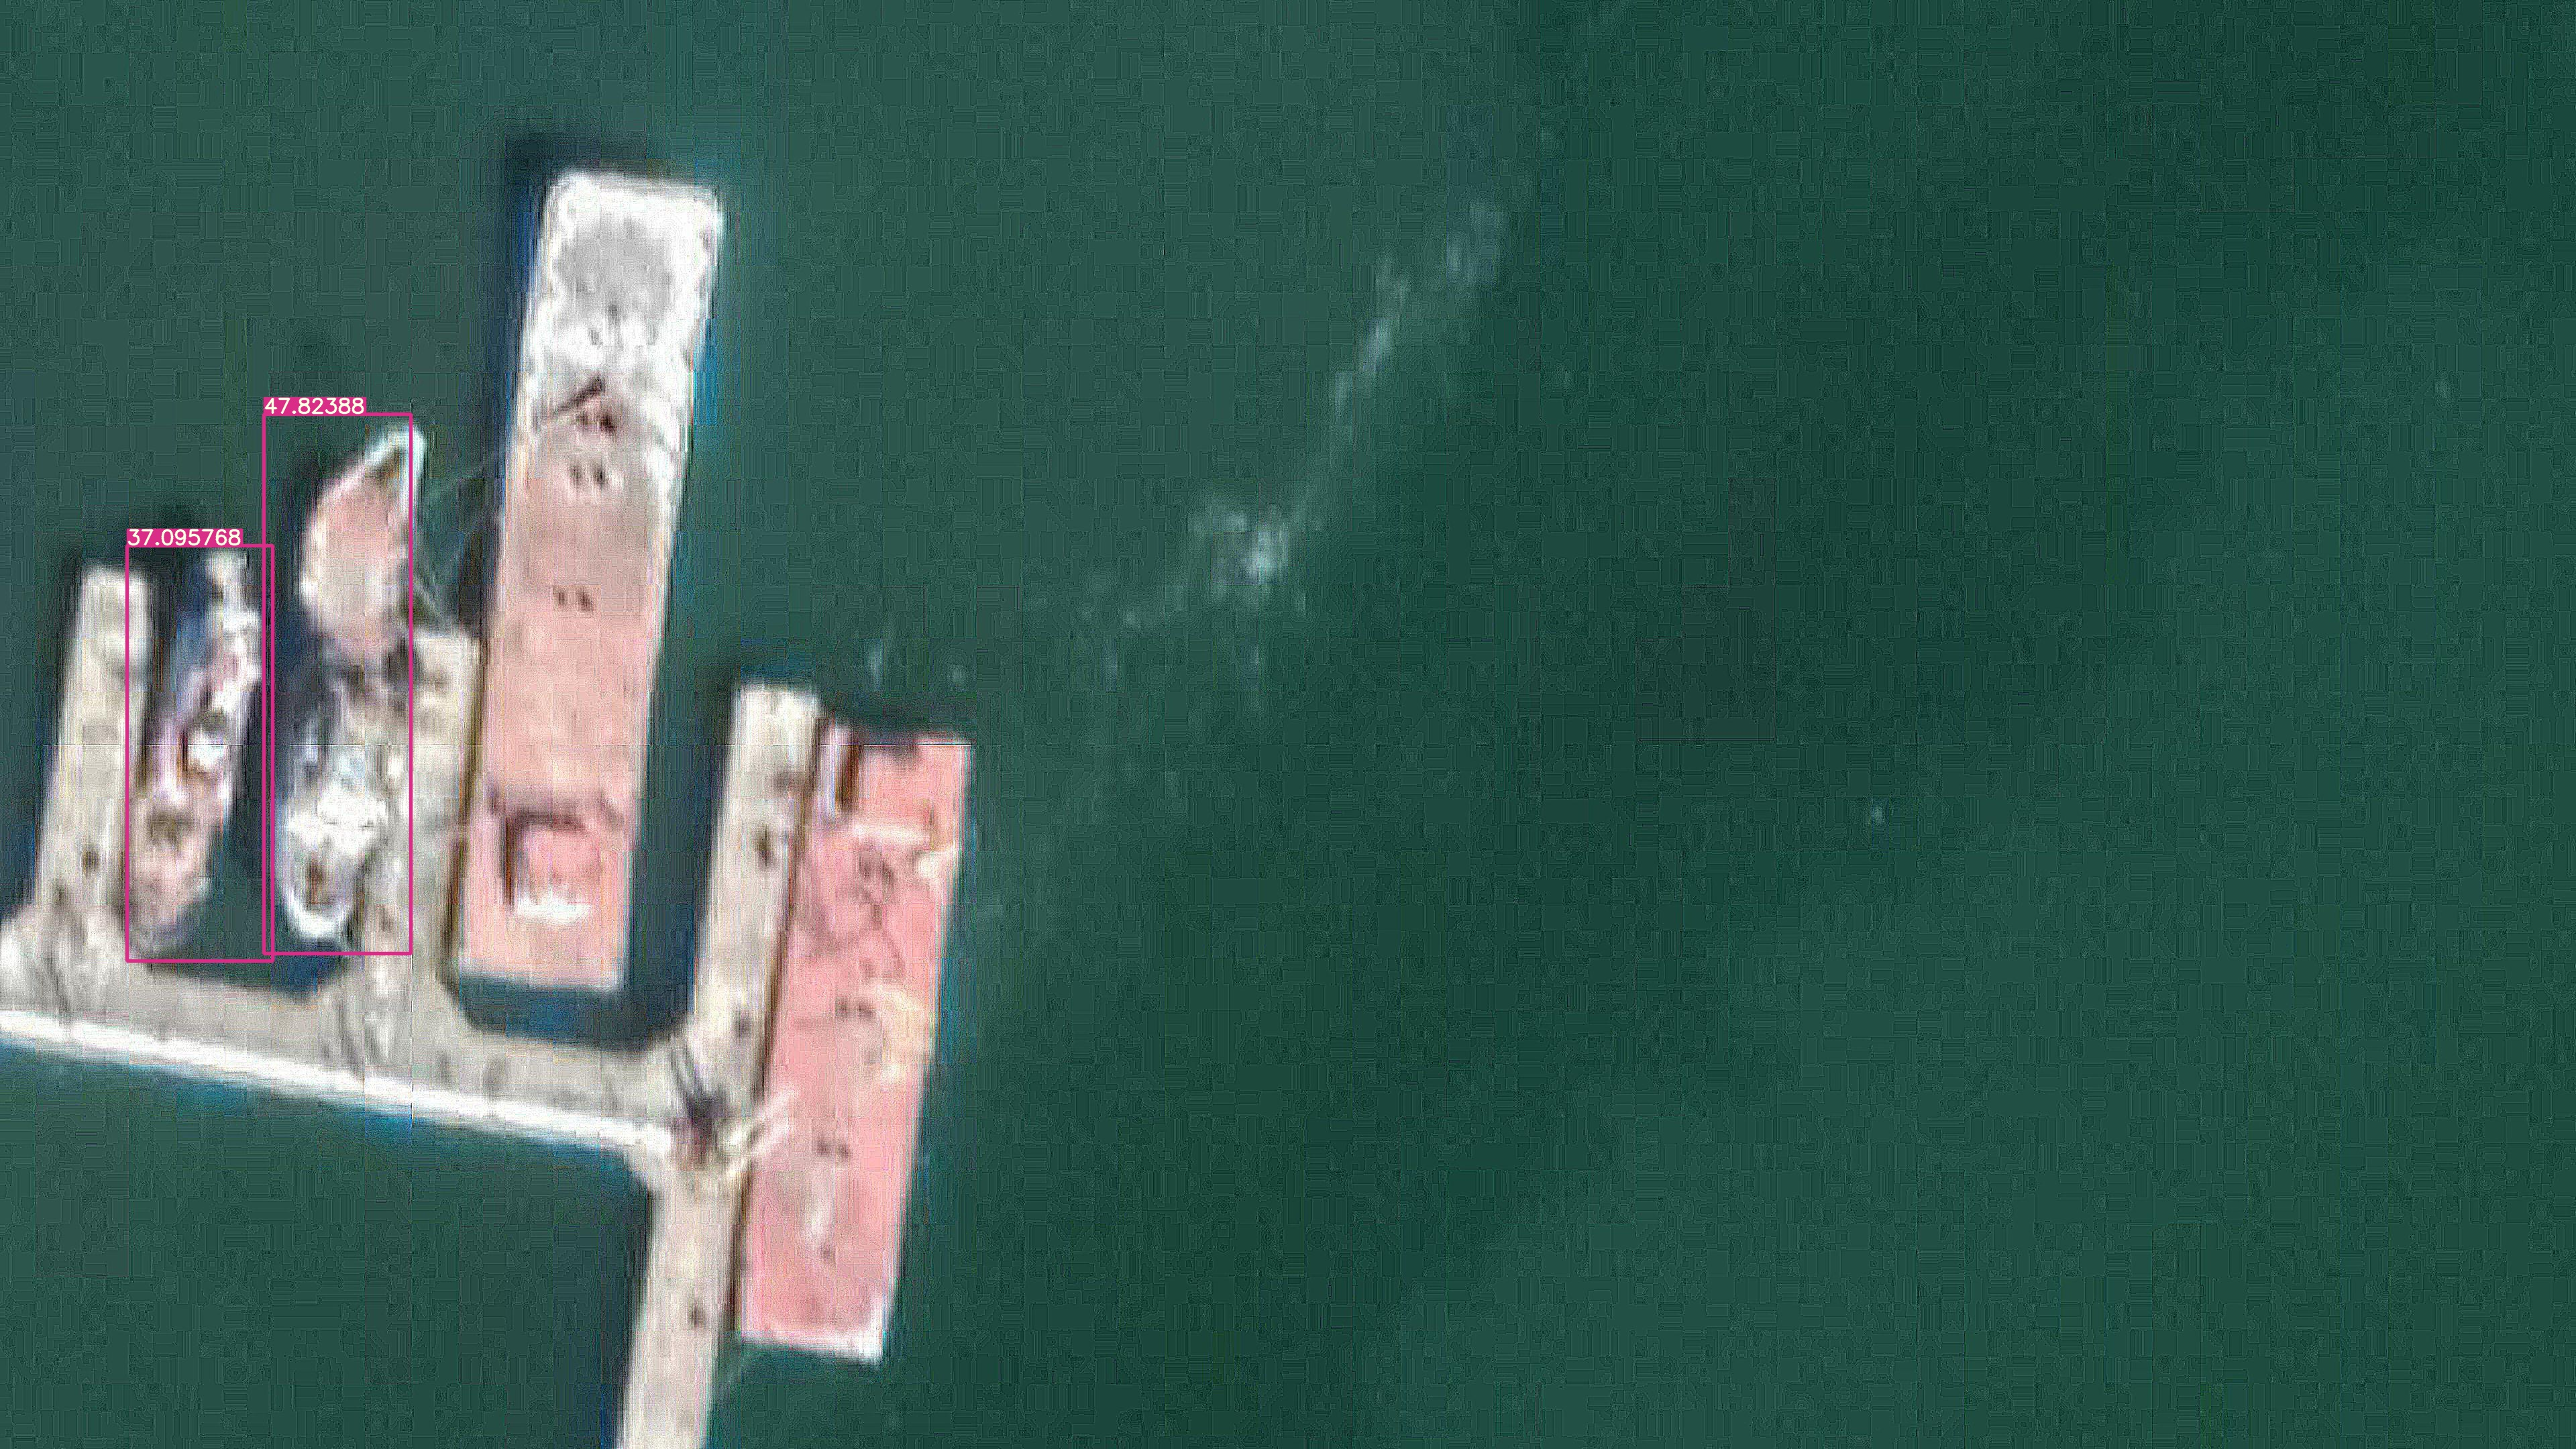
\includegraphics[width=\columnwidth]{img/2_square_Guaymas_202001_01.jpeg}
    \caption{When the cargo ship is full of cargo, the ship looks like a rectangular jetty from above and loses the normal shape of a ship. The image is from Guaymas, January 2020.}
    \label{fig:2_square_Guaymas_202001_01}
\end{figure}

\begin{figure}[t]
    \includegraphics[width=\columnwidth]{img/3_beach_SantaRosalia_202104_02.jpeg}
    \caption{Models may have difficulty detecting small boats moored on the beach. The image is from Santa Rosalia, February 2021.}
    \label{fig:3_beach_SantaRosalia_202104_02}
\end{figure}



\begin{figure}[t]
    \center
    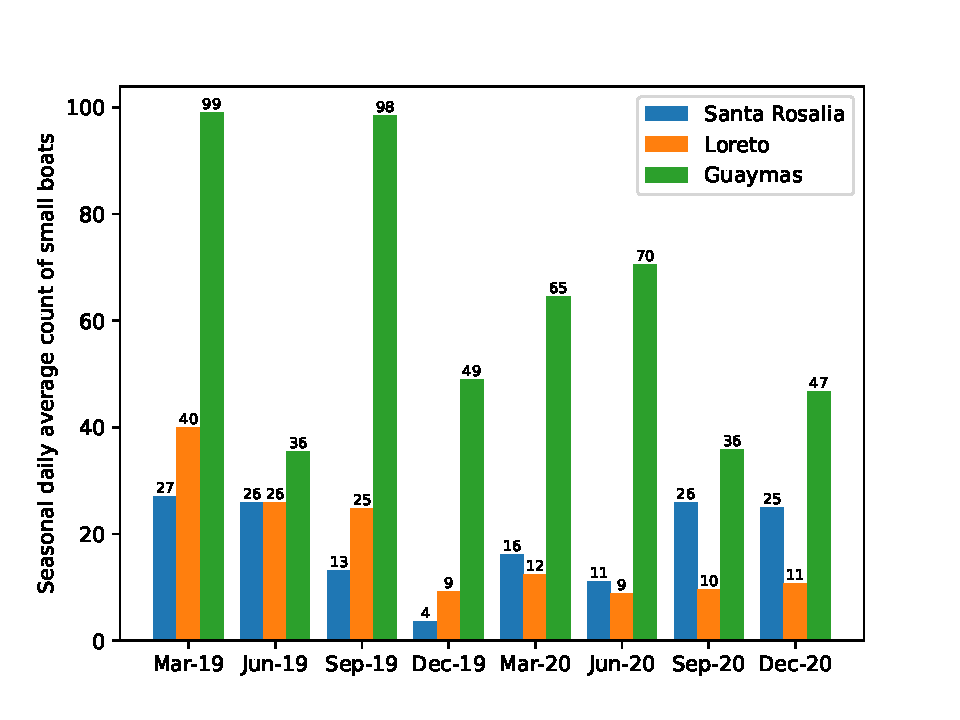
\includegraphics[width=\columnwidth]{img/avg_small.pdf}
    \caption{The seasonal daily average count of small boats in Santa Rosalia, Loreto, and Guaymas between 2019 and 2020.}
    \label{fig:avg_small}

    \center
    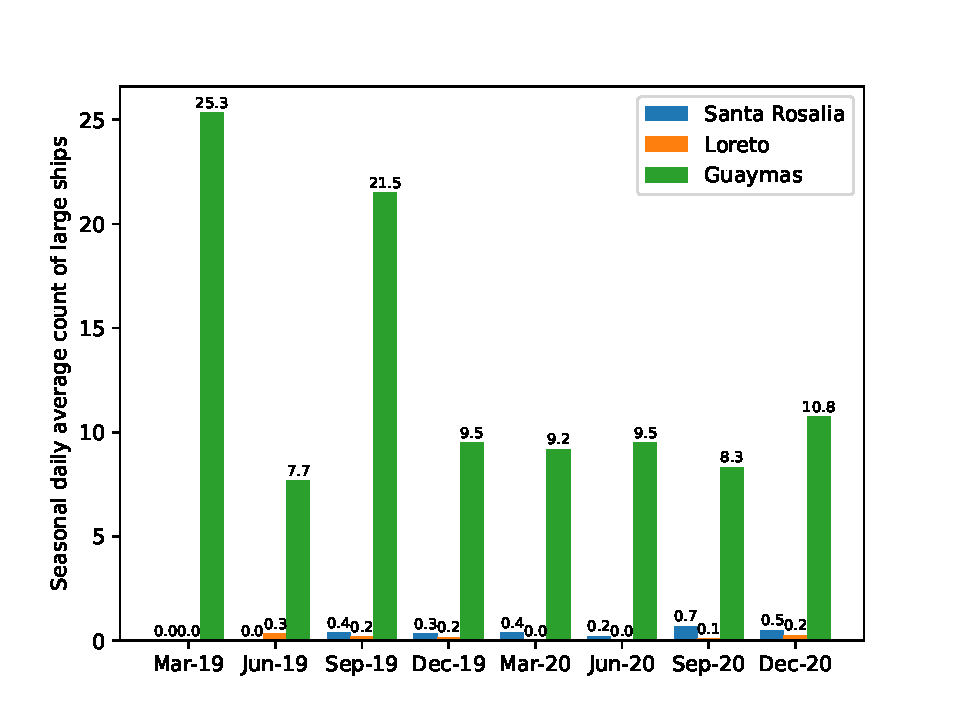
\includegraphics[width=\columnwidth]{img/avg_big.pdf}
    \caption{The seasonal daily average count of large ships in Santa Rosalia, Loreto, and Guaymas between 2019 and 2020.}
    \label{fig:avg_big}
\end{figure}

Nevertheless, as Figures~\ref{fig:1_docked_together_Guaymas_202001_20},~\ref{fig:2_square_Guaymas_202001_01},~\ref{fig:3_beach_SantaRosalia_202104_02} demonstrate, the model still detects most small boats in poorly detailed satellite images, even those images that human eyes cannot easily detect. The number of small and large ships between regions can be seen in Figure~\ref{fig:avg_small} and Figure~\ref{fig:avg_big}. Two different types of port cities can class Guaymas, Loreto and Santa Rosalia:


\begin{enumerate}
    \item Santa Rosalia and Loreto have a much smaller number of small boats and almost no large ships.
    \item The port of Guaymas presented a larger number of small boats when contrasted to the other two coastal cities. There were between 1.37 and 8.00 times more small boats detected in Guaymas than in Santa Rosalia (dependent on the month and year of the image) and 3.00 times more than in Loreto. 
    \item Guaymas had a larger number of large ships as well. There were more than ten times more large ships detected in Guaymas than in Santa Rosalia and Loreto.
    \item In the relatively large seaports of Guaymas and Loreto, there is a tendency for both large and small vessels to decrease with time.
\end{enumerate}

In fact, according to statistic\cite{INEGI2022Population} from the Mexican government, in 2020, the population of Guaymas, Loreto, and Santa Rosalia were 156,863, 18,052, and 14,357, respectively. Therefore, it will seem that the number of detected boats is correlated to the number of habitats, which makes sense since, by probability, there would be more economical and leisure activities around larger coastal cities.


\subsection{Entertainment and Fishing Boats in the Gulf of California}



\begin{table}[t]
\center
\begin{tabular}{|c|c|c|c|c|}
\hline
                                &  Mar-20   & Jun-20    & Sep-20    & Dec-20\\ \hline
   Small boats                  &  323      & 283       & 215       & 187   \\ \hline
   Large ships                  &  46       & 38        & 50        & 43    \\ \hline
   Small white boats            &  302      & 273       & 210       & 174   \\ \hline
   Shipping boats               &  21       & 10        & 5         & 13    \\ \hline
\end{tabular}
\caption{\textbf{Detection example.} Small boats, large ships, and small white boats in Guaymas in 2020.}
\label{Guaymas_2020}
\end{table}

According to the statement in Sec~s\ref{III-D-Detection-Architecture}, determining whether a boat is white can be used as a criterion to determine whether a boat is used for recreation or fishing. As can be seen from Table~\ref{Guaymas_2020}, most of the small boats in Guaymas in 2020 are white ( i.e. all can be classified as recreational boats). However, as discussed before, this conclusion is limited since the algorithm does not consider, for example, other colours as part of the leisure boats. Furthermore, although there are many uncertainties in detecting the colour of the boats, the algorithm also considers situations where the colour of the boats is not fully white due to atmospheric refraction, weather conditions, or cloud interference. The algorithm also considers cases where the boat's colour is light. Therefore, this approach is acceptable from the point of view of algorithm complexity, results, and detecting data quality.



%\section{Future Work}
%Although the location and size of small boats have been successfully identified, and the boats have been successfully but roughly classified into domestic recreational and fishing categories, more work is still needed to refine and improve them. In the future,

\begin{enumerate}
    
    \item in determining whether the boats are white or not, I created a function with RGB as the independent variable. I required the output of this function to be greater than a particular value (threshold). However, adjusting the parameters of this function can, in a certain sense, only be based on experience. So, does this threshold accurately identify the boat as being white in colour?
    
    \item if it is possible to roughly determine the type of small boat based on colour alone, is it possible that a dark coloured fishing boat is not detected on dark coloured seas? Would the number of fishing boats, in fact, then be greater?
    
    \item the satellite images capture only a moment in time during the year, are the fishing vessels operating slightly further out to sea and not captured by the satellite due to the nature of the fishing vessels?


    \item can data providers provide scholars with clear and close satellite imagery for free? Data is one of the triads of artificial intelligence and also the most overlooked factor. In fact, AI algorithms are highly dependent on data. It is as if the algorithms are always hungry, and all need a constant stream of data to feed their hunger. For object detection algorithms, poor image detail representation means less high-quality data. For the algorithm, fewer data often brings poor output results. Therefore, both the data used in building the model and the data used for detection should be kept at the highest level. Otherwise, training AI models loses its relative meaning.
    
    \item will Google Earth Pro provide a deep integration tool about the zoom scale in the future? Google Earth Pro provides very many images with details. However, Google Earth Pro does not offer similar integrated tools for zooming rulers as Google Maps does. If such a scaling environment were available, it would mean that every photo taken on Google Earth Pro would contain its scaling ratio. This means that we do not need to define a fixed zoom scale. It would be easy to know the object's length on each screenshot, regardless of whether the eye altitude is 200 meters or not. This leads to the fact that when some giant cargo ships or cruise ships need to be detected, we can reduce the scale to get an overall picture of the giant ship. When some tiny ships (e.g., a small ship under 5 meters in length) need to be inspected, we can zoom in to get the overall shape of the small ship.
    
    \item will small boats have a more precise classification in the future? Using colour to distinguish whether a boat is a recreational boat or a fishing boat may not be a solution that is acceptable to everyone. However, to solve this problem with a purely deep learning approach, one needs to train the data with all the types of boats that one wants to detect. However, doing the data classification and training in a realistic environment, i.e. Google Earth Pro, would be labour-intensive and costly. Furthermore, when looking for the classification category and the data under this category, is it possible to guarantee that the object‘s environment is the same as the object's environment under other categories due to the AI fairness principle? For example, is it possible to guarantee that the proportion of large cruise ships appearing on the beachside is the same as that of small recreational boats appearing on the beachside? The reason for this is that we do not want all large cruise ships to be offshore and all small recreational boats to be on the beach. If this is the case, the deep neural network does not need to know the contours or characteristics of the different boats. It just needs to analyse the background of the boats (i.e., the colour of the sea level, the colour of the beach, etc.) to predict whether a large cruise ship is likely to be a large cruise ship in the first place. One of the potential solutions to this problem is using computer simulation techniques to create CAD models of various ships. These CAD ships are then placed evenly into a variety of different background environments. Finally, these data are trained with deep neural networks, and then the trained models are put into real-life situations to detect some real ships.
    
    \item *will it be possible in the future to quickly scale up the algorithm to other regions? As well, will it be possible to analyse real-time satellite video in the future? Again, the key to expanding the algorithm to other regions and analysing real-time satellite video is to have fast and timely access to the data in the region. Frankly, it is whether the data providers can provide the data in the region. With real-time satellite video, it will be possible to get a better picture of maritime traffic in any area to monitor and control the carbon emissions of shipping in that area.
    
    \item is it possible to add more recognition objects, such as harbour and sea ripples, to prevent the recognition of harbour or sea ripples as small boats? The purpose of this is that once the algorithm can successfully identify the harbour or sea ripples, they will not be identified as small boats.
    
    \item can the timeframes be better? It is a question of optimisation, a trade-off question on cloud storage, a question of the algorithm's speed, and a question of the accuracy of the result. Besides, can the algorithm distinguish the same boat?
    
    \item Can we get a better idea of the type of engine on the boat? The connection of the ship is rightly allocated but still possible that it is difficult to know what type of engine or power is installed onboard. For this, a better understanding between the ship size and type and the levels of power needed is needed. This suggestion opens a new door of research.
\end{enumerate}
 



%\section{Conclusion}
%
In this study, I introduce the reader to satellite image recognition and how I can make a modest contribution to the development of the field.

In Chapter~\ref{chap:2}, I review the traditional research literature on estimating the number of small boats. Researchers use kernel density estimation to distribute population and vessel numbers and ultimately show that their predictions can accurately predict the number of vessels in the Gulf fisheries. Some scholars then focused on describing the combination of national small vessel registries and surveyed vessel discharge results. However, the methodology does not cover states without a national small boat registry, and small boats are not just recreational vessels.

Obviously, these traditional approaches do not extract information well from a large amount of data. Although as early as the 1990s, researchers such as Yann LeCun realized that convolutional neural networks could recognise images. However, with the exponential growth in computing power in the last five years, scientists and engineers have only been able to apply convolutional neural networks to topics such as large-scale image recognition and object detection. Since 2012, the field has been reinvented by creating large-scale supervised datasets and developing neural object detection network models. Although it has only been nine years since then, the field has evolved at an amazing rate. Innovations in building better datasets and more effective models have alternated, and both have contributed to the field's growth.

In Chapter~\ref{chap:3}, I first explain how convolutional neural networks can detect a letter `X' and describe the mathematical principles involved. Next, I introduce the two most commonly used neural network frameworks today: Faster RCNN and YOLO and cite Dwivedi's work to illustrate to the reader the advantages of the YOLO model in recognising small objects advantage of higher accuracy in recognising objects in videos. Next, I show the data needed in training the model and the preparation needed to train the model faster. Finally, to speed up the model's training, I use a GPU to train the model and use Google Colab, Google Drive and GitHub as my testing and development tools.


In the subsequent section, I highlight the inequality in the amount of data available on satellite images for the Gulf of California. Thus, I took the approach of selecting one of the cities with a large amount of satellite data every year and then analysing it. However, even this does not avoid the fact that the quality of the satellite images in 2019 is worse compared to the following two years. In response, I took the approach of sharpening the images to bring out the details of the images. As a result, the model can improve the object recognition rate by around 26\%.

Then, I designed algorithms to detect the length of small boats. Since I did not have access to the zoom scale of Google Earth Pro, I had to define a zoom scale myself to find the relationship between the length of the real boat and the boat in the image. Finally, by using the same eye altitude and resolution for all the photos in the test dataset, the algorithm can automatically detect the boat's length. In the test, the boat's length detected by the algorithm is similar to the length measured from Google Earth Pro.

In Chapter~\ref{chap:4}, I show the detection results that can combine open high-resolution satellite data and convolutional neural networks. The results are not as high as the ideal recognition rate, but such detection results are still acceptable due to the inferior quality of the monitoring data. 

The results show a divergence. In 2019, there were on average 100.63 small boats in Guaymas. Although this value dropped to 91.55 in 2020, it quickly rises again to 147.75 in 2021. Similarly, in 2019, 2020 and 2021, there are 31, 46.55 and 39 small boats in Santa Rosalia, respectively. However, Loreto did not show such an upward trend in general. In 2019, 2020 and 2021, there are 37.13, 29.22 and 27.33 small boats in Loreto, respectively. On the one hand, there is a large port like Guaymas with many small ships. On the other hand, small ports like Loreto and Santa Rosalia have almost no big ships and fewer small ships. But it is interesting to note that small boats in Guaymas, Loreto and Santa Rosalia are almost certainly small boats for family use for recreation. The analysis of satellite images shows that most small boats are docked in the harbour, which means it is rare to see a large number of small boats floating on the sea. Another interesting point is that the number of small boats identified increases as the year increases. Considering that most of the boats are in the harbour and that the models used for the tests are identical, the only difference is that the detail of the satellite images is better realisable each year, i.e., each year we have an image with higher quality. Then, it is reasonable to believe that the increase in the quality of satellite photos can improve the quality of object detection.



% 4. Include a brief reflection on what I have learnt from undertaking my project as far as project management is concerned.
 
%\section{Brief Reflection}
All in all, I am very excited about the progress I have made in this area over the past four months and are pleased to contribute to the field. At the same time, I am convinced that there is still a long way to get AI to the point where it can detect objects beyond the human level, and we still face huge challenges and many outstanding questions that need to be addressed in the future. One key challenge is that we still do not have a good way to handle deeper object detection ---- those problems that require understanding photos or video inference ---- for example, the question of whether the two boats are one boat. In the future, we will also have to address the complex problem of integrating object detection and natural language processing to reach a level that allows AI to understand video.

We also hope to encourage more researchers to work on applying satellite image detection to new areas. We believe it will lead us to build better agents that can understand media and hope to see these ideas implemented and developed in industry applications.

\section{Discussion}

This study demonstrated the capabilities of a deep learning approach for the automatic detection and identification of small boats in the waters surrounding three cities in the Gulf of California with a precision of up to 74.0\%. This work used CNNs to identify types of small vessels. Specifically, this study presented an image detection model, BoatNet, capable of distinguishing small boats in the Gulf of California with an accuracy of up to 93.9\% and encouraging results considering the high variability of the input images.

Even with the model level of performance using large and highly ambiguous training images, it was found that image sharpening improved model accuracy. This implies that access to better quality imagery, such as that available through paid for services, should considerably improve model precision and training times.

The results of this research have several important implications. First, the study used satellite data to predict the number and types of ships in three important cities in the Gulf of California. The resulting analysis can contribute to the region's shipping fleet composition, level of activity and ultimately their carbon inventory by adding the emissions produced by the small boat fleet. Further, through this approach, it is also possible to assign emissions into regions supporting the development of policies that can mitigate local GHG and air pollution. In addition, the transfer learning algorithm can be pre-trained in advance and immediately applied to any sea area worldwide. This will provide a potential method to increase efficiency for scientists and engineers worldwide who need to estimate local maritime emissions. In addition, the model can quickly and accurately identify the boat's length and classify them, allowing researchers to allocate more time to the vessels they need concentrate on, not just small boats. Finally, all of the above benefits can be exploited in under served areas with a shortage of infrastructure and resources.

This work is the first step to building emission inventories through image recognition, and it has some limitations. The study considered the ship as a single detection object. It did not evaluate whether the model can improve the accuracy of identifying ships in the case of multiple detection objects. For instance, BoatNet was not trained to detect docks to improve the metrics of detecting boats. By down-sampling the image to 416 pixels × 416 pixels, it is possible to mask some of the boats at the edges of the photograph.
Furthermore, deep learning models train faster on small images~\cite{tan2021efficientnetv2}. A larger input image requires the neural network to learn from four times as many pixels, increasing the architecture's training time. In this work, a considerable proportion of the images in the dataset were large images of 4800 pixels x 2908 pixels. Thus, BoatNet was set to learn from resized small images measuring 416 pixels x 416 pixels. Due to the low data quality of the selected regions, the images are less suitable as training datasets. However, using datasets from other regions or higher quality open-source imagery may result in inaccurate coverage of all types of ships in the region. When focusing on the small boat categorisation and the data used, understanding the implications of different environments (e.g. water or land) on object classification accuracy through the AI fairness principle deserves further study. From this point of view, large-scale collection of data sources in the real physical world would be costly and time-consuming. That said, it is possible that reinforcement learning, or building simulations in the virtual world, could reduce the negative impact of the environment on object recognition and thus improve its categorisation precision. Of all these limitations, model detection still achieves excellent performance in detecting and classifying small boats.

It is important to remember that BoatNet currently only detects and classifies certain types of small boats. Therefore, to estimate fuel consumption and emissions, it is necessary to couple it with small boat behaviour datasets~\cite{ferrer2021mexican}, typical machinery, fuel characteristics, and emission factors unique to this maritime segment~\cite{inecc2020inventario}. 

Finally, this work has demonstrated that deep learning models have the potential to identify small boats in extreme environments at performance levels that provide practical value. With further analysis and small boat data sources, these methods may eventually allow for the rapid assessment of shipping carbon inventories.



% References section
\bibliographystyle{IEEEtran}
\bibliography{bibliography}


\section{Biography Section}
%If you have an EPS/PDF photo (graphicx package needed), extra braces are needed around the contents of the optional argument to biography to prevent the LaTeX parser from getting confused when it sees the complicated
% $\backslash${\tt{includegraphics}} command within an optional argument. (You can create
% your own custom macro containing the $\backslash${\tt{includegraphics}} command to make things
% simpler here.)
 
\vspace{11pt}
\textbf{Guo Jialeng} received the MSc degree in Energy System and Data Analytics from University College London (UCL) in 2021 and the BEng degree in Electronic Engineering from the University of Leeds in 2019. In computer vision, his interests include understanding and developing energy and climate systems with human-centred object detection and learning system.

\textbf{Dr Santiago Suárez de la Fuente} is Lecturer in Energy and Transport at University College London (UCL) Energy Institute. His research focuses on marine energy-efficient technologies, holistic modelling approaches for the maritime sector, performance data analytics and decarbonization pathways for shipping. He is currently working on finding feasible and equitable business opportunities in developing nations to transition the maritime sector. Dr Suarez de la Fuente did his PhD at UCL on marine waste heat recovery systems (WHRS). He was granted the Institute of Marine Engineering, Science and Technology (IMarEST) Stanley Gray fellowship and the prestigious Denny Medal. He studied his bachelor’s degree in Mechanical Engineering at the Institute of Technology and Higher Education (ITESO, Mexico). He has an MSc degree in Mechanical Engineering at UCL (2010-2011).


%\bf{If you include a photo:}\vspace{-33pt}
%\begin{IEEEbiography}[{\includegraphics[width=1in,height=1.25in,clip,keepaspectratio]{fig1}}]{Michael Shell}
%Use $\backslash${\tt{begin\{IEEEbiography\}}} and then for the 1st argument use $\backslash${\tt{includegraphics}} to declare and link the author photo.
%Use the author name as the 3rd argument followed by the biography text.
%\end{IEEEbiography}





\vfill

\end{document}


